\documentclass[AnalisiDeiRequisiti.tex]{subfiles}

\begin{document}

\chapter{Casi d'uso}
\section{Attori dei casi d'uso}
\subsection{Attori primari}
\begin{enumerate}
	\begin{figure}[h]
		\centering
		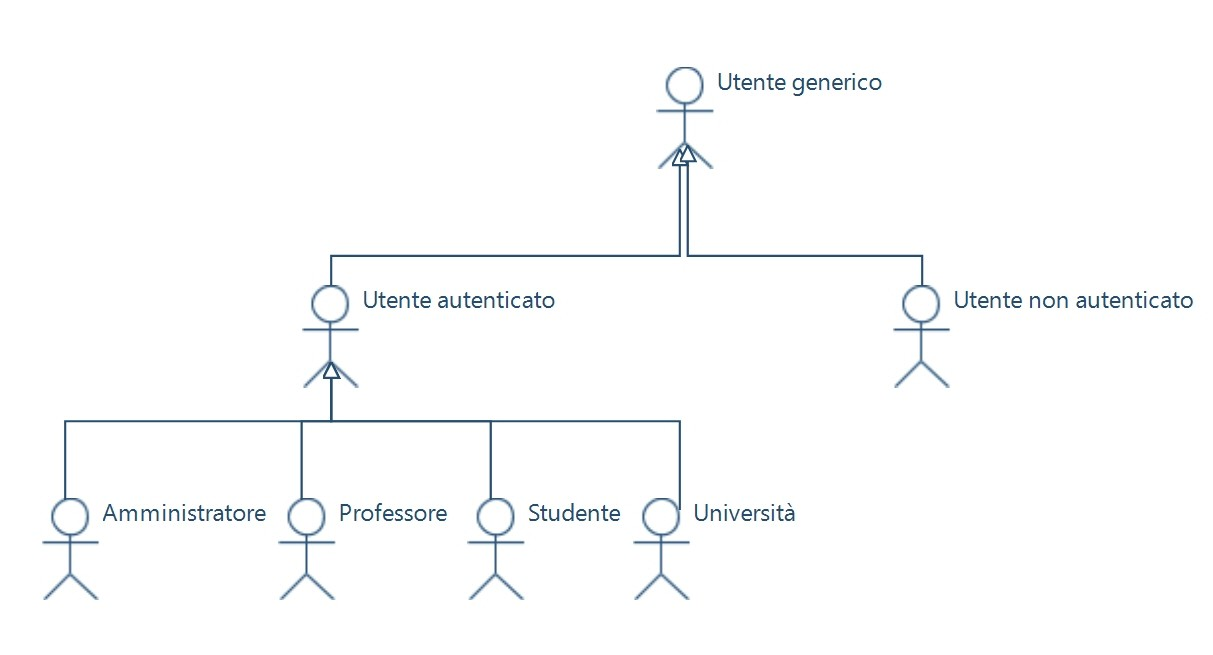
\includegraphics[width=0.8\linewidth]{attoriPrincipali.jpg}
		\caption{Gerarchia attori primari}
		\label{fig:Gerarchia attori primari}
	\end{figure}
	
	\item \textbf{Utente generico}\\
	Si riferisce ad un utente generico che accede al sito\\
	
	\item \textbf{Utente non autenticato}\\
	Ci si riferisce ad un utente generico con non ha ancora effettuato il login.\\
	
	\item \textbf{Utente autenticato}\\
	 Ci si riferisce ad un utente generico con chiave valida ed autenticato nel sistema tramite la procedura di login.\\
	
	\item \textbf{Amministratore}\\
	Ci si riferisce ad un utente autenticato nel sistema nel ruolo di amministratore, ha i permessi per gestire i professori.\\
	
	\item \textbf{Professore}\\
	Ci si riferisce ad un utente autenticato nel sistema nel ruolo di professore.\\
	
	\item \textbf{Studente}\\
	Ci si riferisce ad un utente autenticato nel sistema nel ruolo di studente.\\
		
	\item \textbf{Università}\\
	Ci si riferisce ad un utente autenticato nel sistema nel ruolo di fondatore e rappresentante dell'università, ha i permessi per gestire gli amministratori.\\	
\end{enumerate}

\subsection{Attori secondari}
\begin{enumerate}
	\item \textbf{\citGloss{MetaMask}}\\
	Plugin del \citGloss{browser} \citGloss{MetaMask} per interfacciarsi ad una rete \citGloss{Ethereum}.\\
	
	\item \textbf{Ufficio Universitario}\\
	Entità fisica che consente l'immatricolazione e la registrazione dei professori.\\
\end{enumerate}

\section{Elenco dei casi d'uso}

\begin{figure}[H]
	\centering
	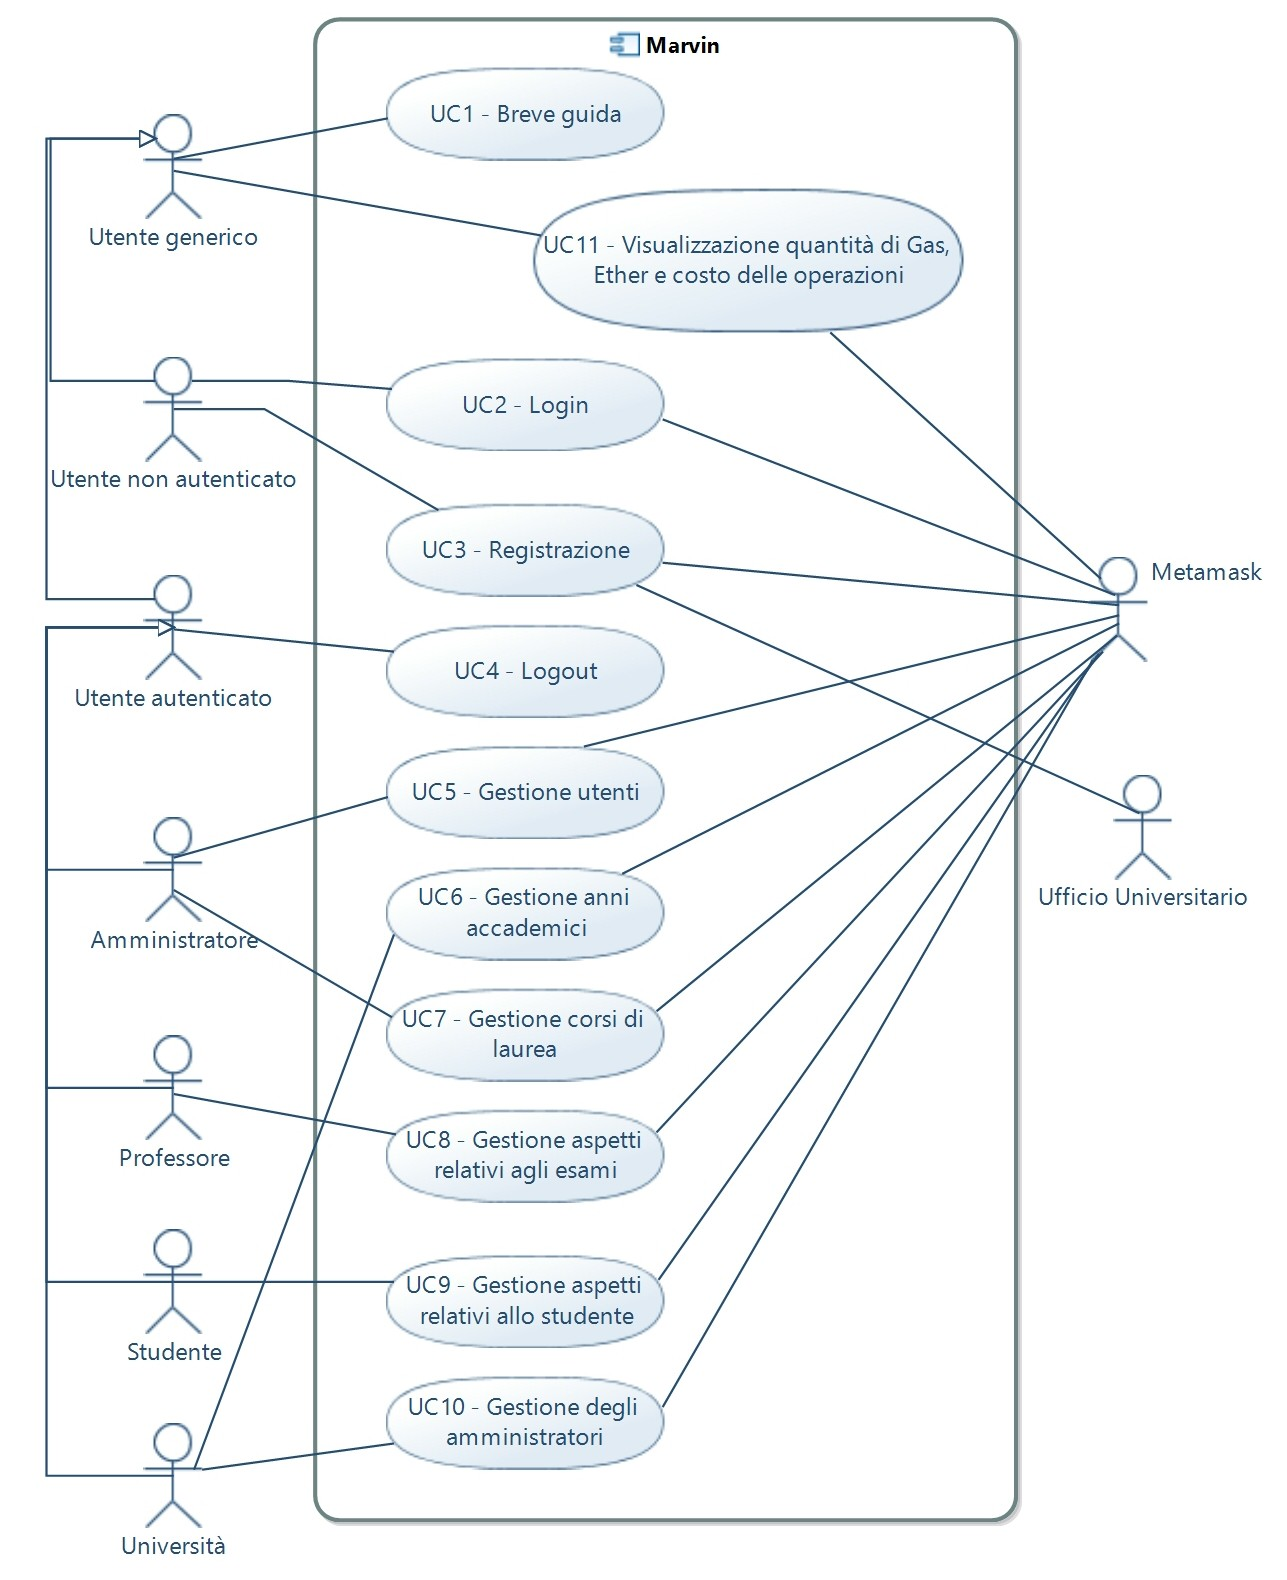
\includegraphics[width=0.8\linewidth]{UC.jpg}
	\caption{Casi d'uso basilari}
	\label{fig:Casi d'uso basilari}
\end{figure}

%   -------------------------------------------------------------------------------------
%   ----------                 MODELLO PER GLI USER CASE              -------------------
%   -------------------------------------------------------------------------------------
\begin{comment}
\subsection{UCX - Nome}
\begin{itemize}
	\item \textbf{Attori primari:} ;\\
	\item \textbf{Attori secondari:} ;\\
	\item \textbf{Scopo e descrizione:} ;\\
	\item \textbf{Scenario principale:} ;\\
	\item \textbf{Scenario alternativo:} ;\\
	\item \textbf{Flusso principale degli eventi:};\\
	\begin{enumerate}
		\item L'utente... ;
		\item L'utente... ;
	\end{enumerate}
	\item \textbf{Estensioni:}\\
		\begin{enumerate}
		\item Se l'utente... ;[UCX.X.X]
	\end{enumerate}
	\item \textbf{Precondizione:} ;\\
	\item \textbf{Postcondizione:} .\\
\end{itemize}
\end{comment}
%

%TODO: decidere se le sottoliste devono avere il ; finale oppure no
\subsection{UC1 - Breve guida}
\begin{itemize}
	\item \textbf{Attori primari:} utente generico;\\
	\item \textbf{Scopo e descrizione:} l'utente visualizza una breve guida di introduzione su come installare il plugin \citGloss{MetaMask} e su come gestire le chiavi in modo da istruirlo sulle modalità di accesso al sistema;\\
	\item \textbf{Scenario principale:} l'utente accede alla guida;\\
	\item \textbf{Precondizione:} il sistema è raggiungibile e funzionante e l'utente desidera aprire la guida;\\
	\item \textbf{Postcondizione:} l'utente ha avuto delle nozioni riguardanti l'accesso al sistema.\\
\end{itemize}
\subsection{UC2 - Login}
\begin{itemize}
	\item \textbf{Attori primari} utente non autenticato;\\
	\item \textbf{Attori secondari:} \citGloss{MetaMask};
	\item \textbf{Scopo e descrizione:} l'utente richiede il login al sistema attraverso il plugin \citGloss{MetaMask};\\
	\item \textbf{Scenario principale:} l'utente non ancora riconosciuto dal sistema effettua il login;\\
	\item \textbf{Precondizione:} l'utente non è stato riconosciuto dal sistema;\\
	\item \textbf{Postcondizione:} l'utente viene riconosciuto da parte del sistema.\\
\end{itemize}

\begin{figure}[H]
	\centering
	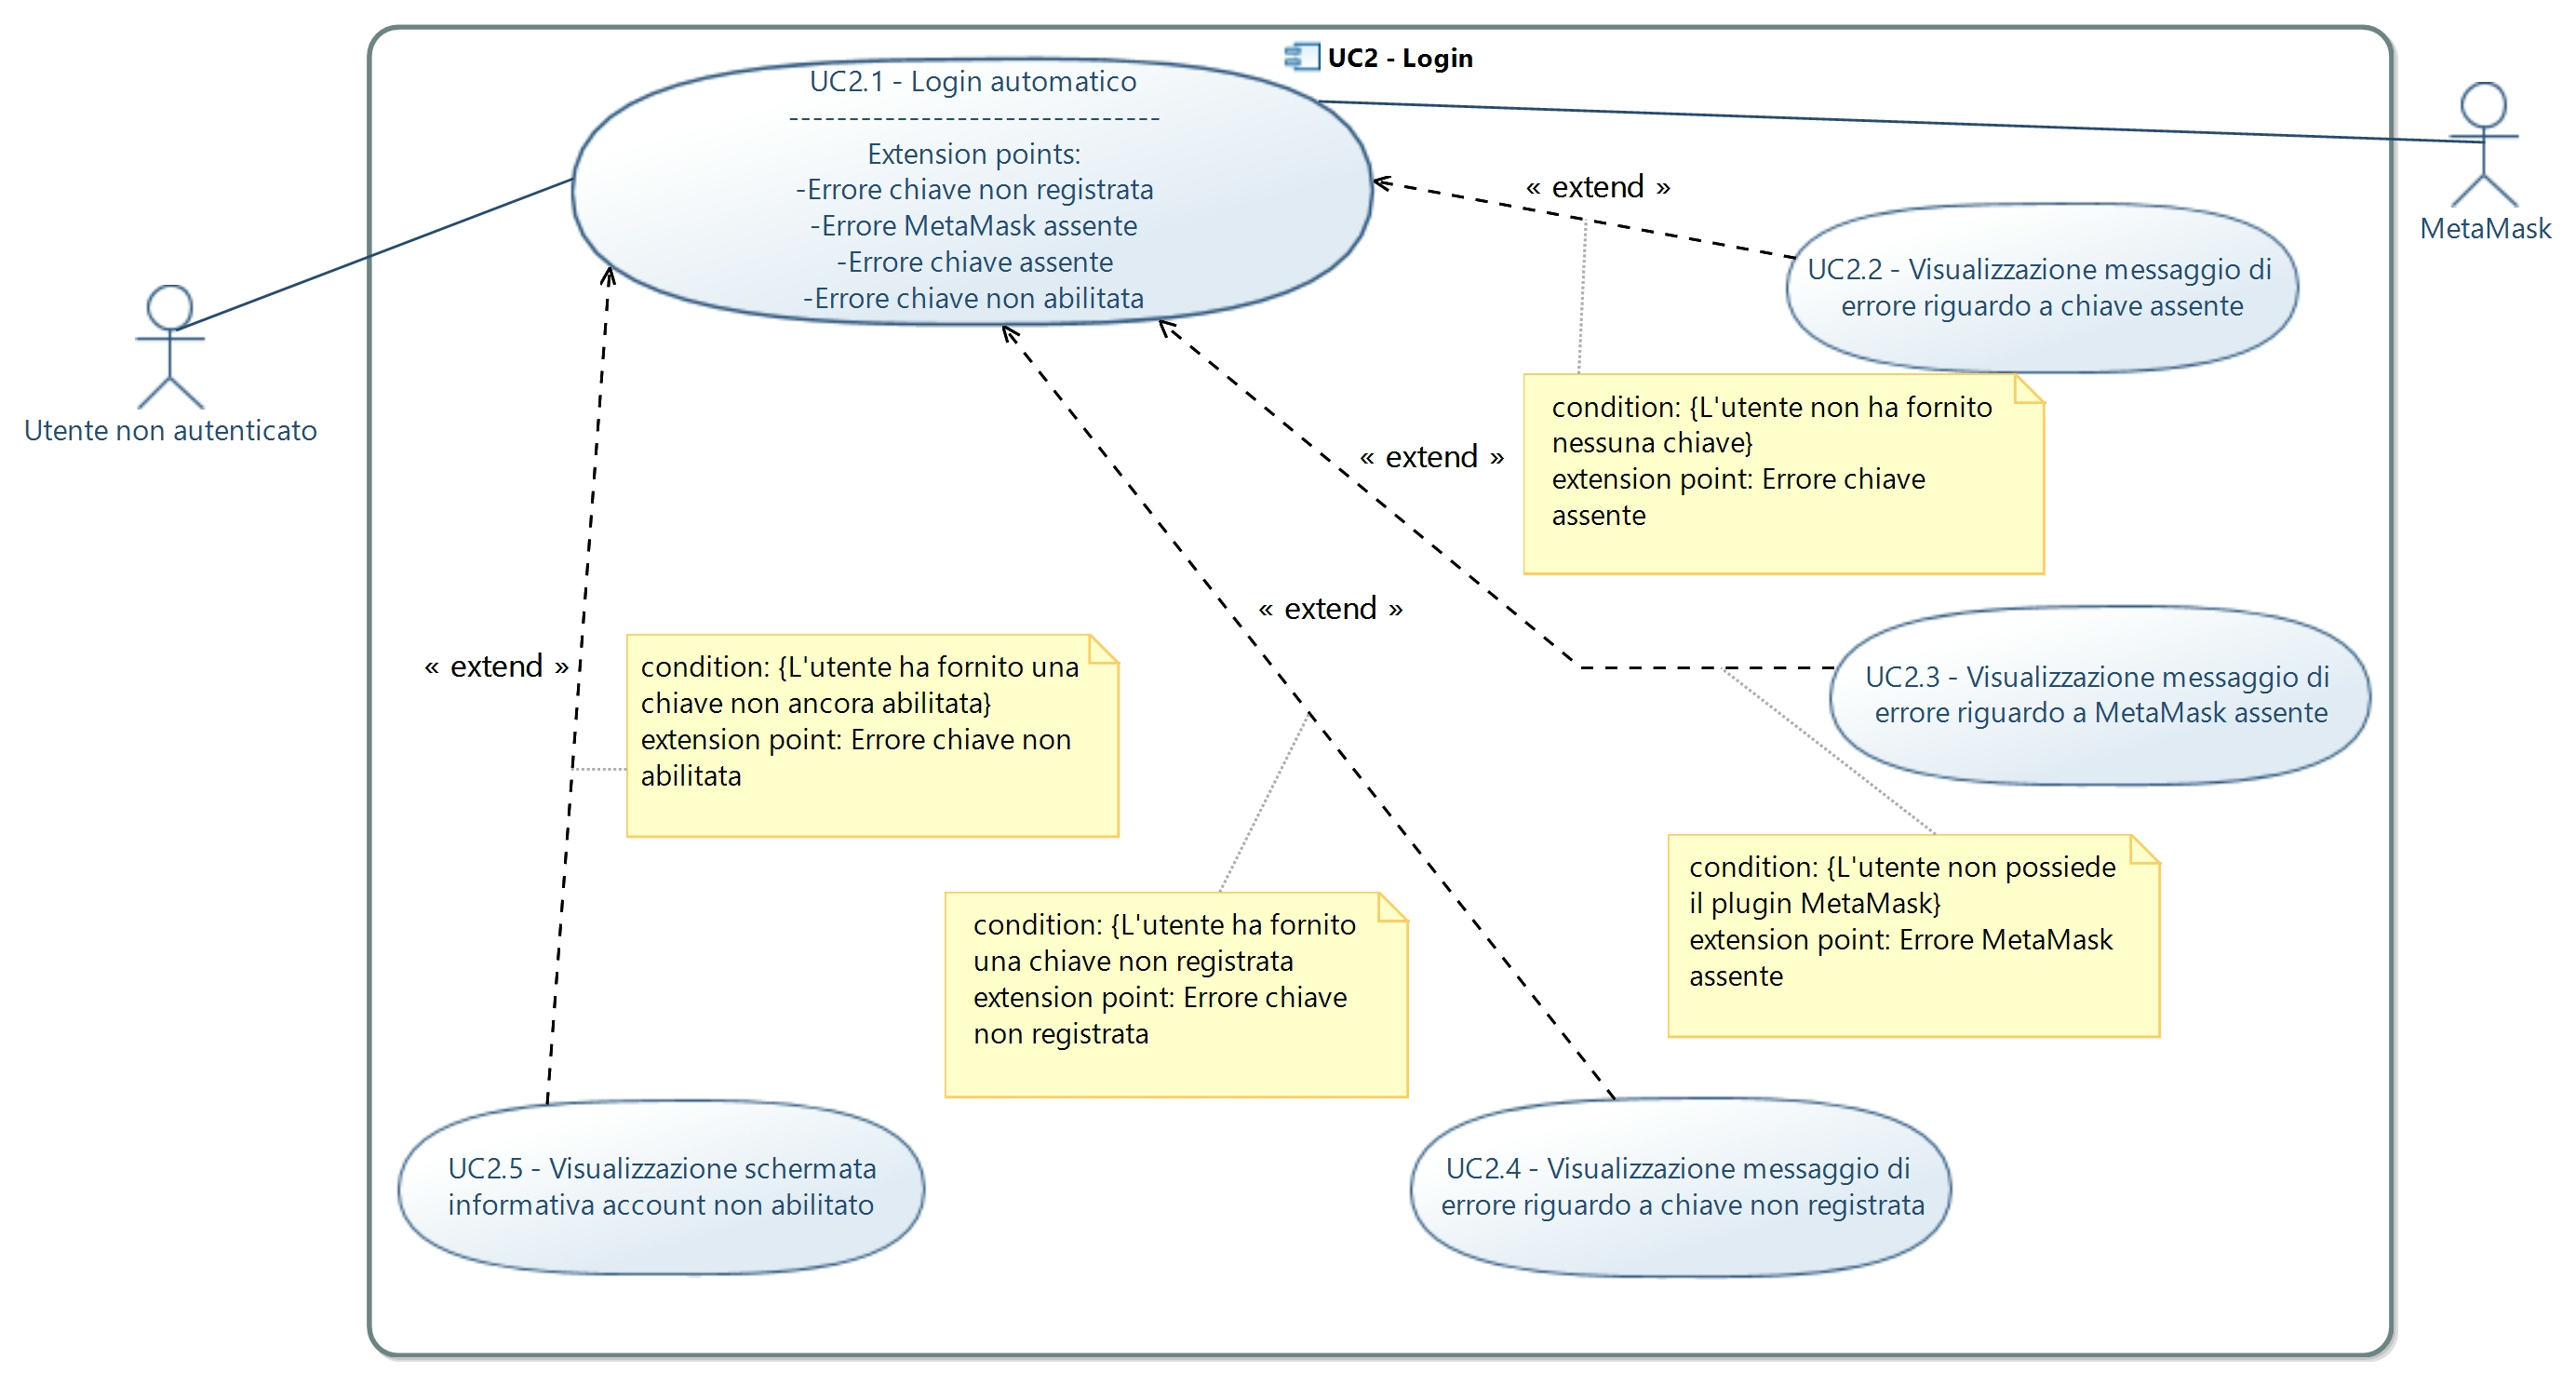
\includegraphics[width=1.0\linewidth]{UC2.jpg}
	\caption{UC2 - Login}
	\label{fig:UC2 - Login}
\end{figure}

\subsection{UC2.1 - Login automatico}
\begin{itemize}
\item \textbf{Attori primari} utente non autenticato;\\
\item \textbf{Attori secondari:} MetaMask;\\
\item \textbf{Scopo e descrizione:} l'utente attende il login da parte del sistema senza effettuare nessuna operazione aggiuntiva;\\
\item \textbf{Scenario principale:} l'utente non ancora riconosciuto dal sistema richiede il login;\\
\item \textbf{Estensioni:}\\
\begin{enumerate}
	\item se l'utente non ha a disposizione una chiave viene avvisato con un errore a riguardo [UC2.2];
	\item se l'utente ha a disposizione una chiave malformata viene avvisato con un errore a riguardo [UC2.3];
	\item se l'utente ha a disposizione una chiave non registrata viene avvisato con un errore a riguardo [UC2.4];
	\item se l'utente tenta di fare il login con un account in attesa d'informazione viene avvisato con una schermata informativa a riguardo [UC2.5].
\end{enumerate}
\item \textbf{Precondizione:} l'utente ha richiesto al sistema di venire riconosciuto;\\
\item \textbf{Postcondizione:} l'utente viene riconosciuto da parte del sistema.\\
\end{itemize}
\subsection{UC2.2 - Visualizzazione messaggio di errore riguardo a chiave assente}
\begin{itemize}
	\item \textbf{Attori primari:} utente non autenticato;\\
	\item \textbf{Scopo e descrizione:} l'utente viene avvisato del fatto che non ha fornito nessuna chiave al sistema;\\
	\item \textbf{Scenario principale:} l'utente visualizza l'errore relativo all'assenza di una chiave per accedere al sistema;\\
	\item \textbf{Precondizione:} l'utente richiede il login senza fornire una chiave;\\
	\item \textbf{Postcondizione:} l'utente è consapevole di dover fornire una chiave. \\
\end{itemize}
\subsection{UC2.3 - Visualizzazione messaggio di errore riguardo a chiave malformata}
\begin{itemize}
	\item \textbf{Attori primari:} utente non autenticato;\\
	\item \textbf{Scopo e descrizione:} l'utente viene avvisato del fatto che ha fornito una chiave malformata, quindi con lunghezza invalida o contenente caratteri non permessi;\\
	\item \textbf{Scenario principale:} l'utente visualizza il messaggio d'errore relativo alla chiave malformata;\\
	\item \textbf{Precondizione:} l'utente richiede il login utilizzando una chiave malformata;\\
	\item \textbf{Postcondizione:} l'utente è consapevole di cambiare la chiave o sistemare quella fornita.\\
\end{itemize}
\subsection{UC2.4 - Visualizzazione messaggio di errore riguardo a chiave non registrata}
\begin{itemize}
	\item \textbf{Attori primari:} utente non autenticato;\\
	\item \textbf{Scopo e descrizione:} l'utente viene avvisato del fatto che ha fornito una chiave non registrata nel sistema;\\
	\item \textbf{Scenario principale:} l'utente viene informato che la sua chiave non risulta registrata, suggerendone la registrazione;\\
	\item \textbf{Precondizione:} l'utente richiede il login utilizzando una chiave non registrata;\\
	\item \textbf{Postcondizione:} l'utente è consapevole di dover effettuare la registrazione per accedere al sistema.\\
\end{itemize}
\subsection{UC2.5 - Visualizzazione schermata informativa account non abilitato}
\begin{itemize}
	\item \textbf{Attori primari:} utente non autenticato;
	\item \textbf{Scopo e descrizione:} l'utente viene informato che la sua chiave non è ancora stata abilitata all'uso dei servizi;
	\item \textbf{Scenario principale:} il sistema mostra una schermata informativa per avvisare l'utente che il suo account è in attesa di essere abilitato;
	\item \textbf{Precondizione:} l'utente tenta di accedere al sistema senza che il suo account sia stato abilitato; 
	\item \textbf{Postcondizione:} l'utente è consapevole di aspettare l'abilitazione del suo account per accedere al sistema.
\end{itemize}
\subsection{UC3 - Registrazione}
\begin{itemize}
	\item \textbf{Attori primari:} utente non autenticato;\\
	\item \textbf{Attori secondari:} \citGloss{MetaMask}, Ufficio Universitario;
	\item \textbf{Scopo e descrizione:} l'utente non autenticato compila i campi richiesti per registrarsi nel sistema, successivamente si dovrà presentare all'ufficio universitario con i documenti per l'identificazione;\\
	\item \textbf{Scenario principale:}
	\begin{enumerate}
		\item l'utente inserisce il suo nome [UC3.1];
		\item l'utente inserisce il suo cognome [UC3.2];
		\item l'utente seleziona la sua categoria [UC3.3];
		\item l'utente seleziona il corso desiderato [UC3.4].
	\end{enumerate}
	\item \textbf{Precondizione:} l'utente è entrato nel sistema e ha scelto di registrarsi;\\
	\item \textbf{Postcondizione:} la registrazione è andata a buon fine e la chiave dell'utente è stata salvata nel sistema.\\
\end{itemize}

\begin{figure}[H]
	\centering
	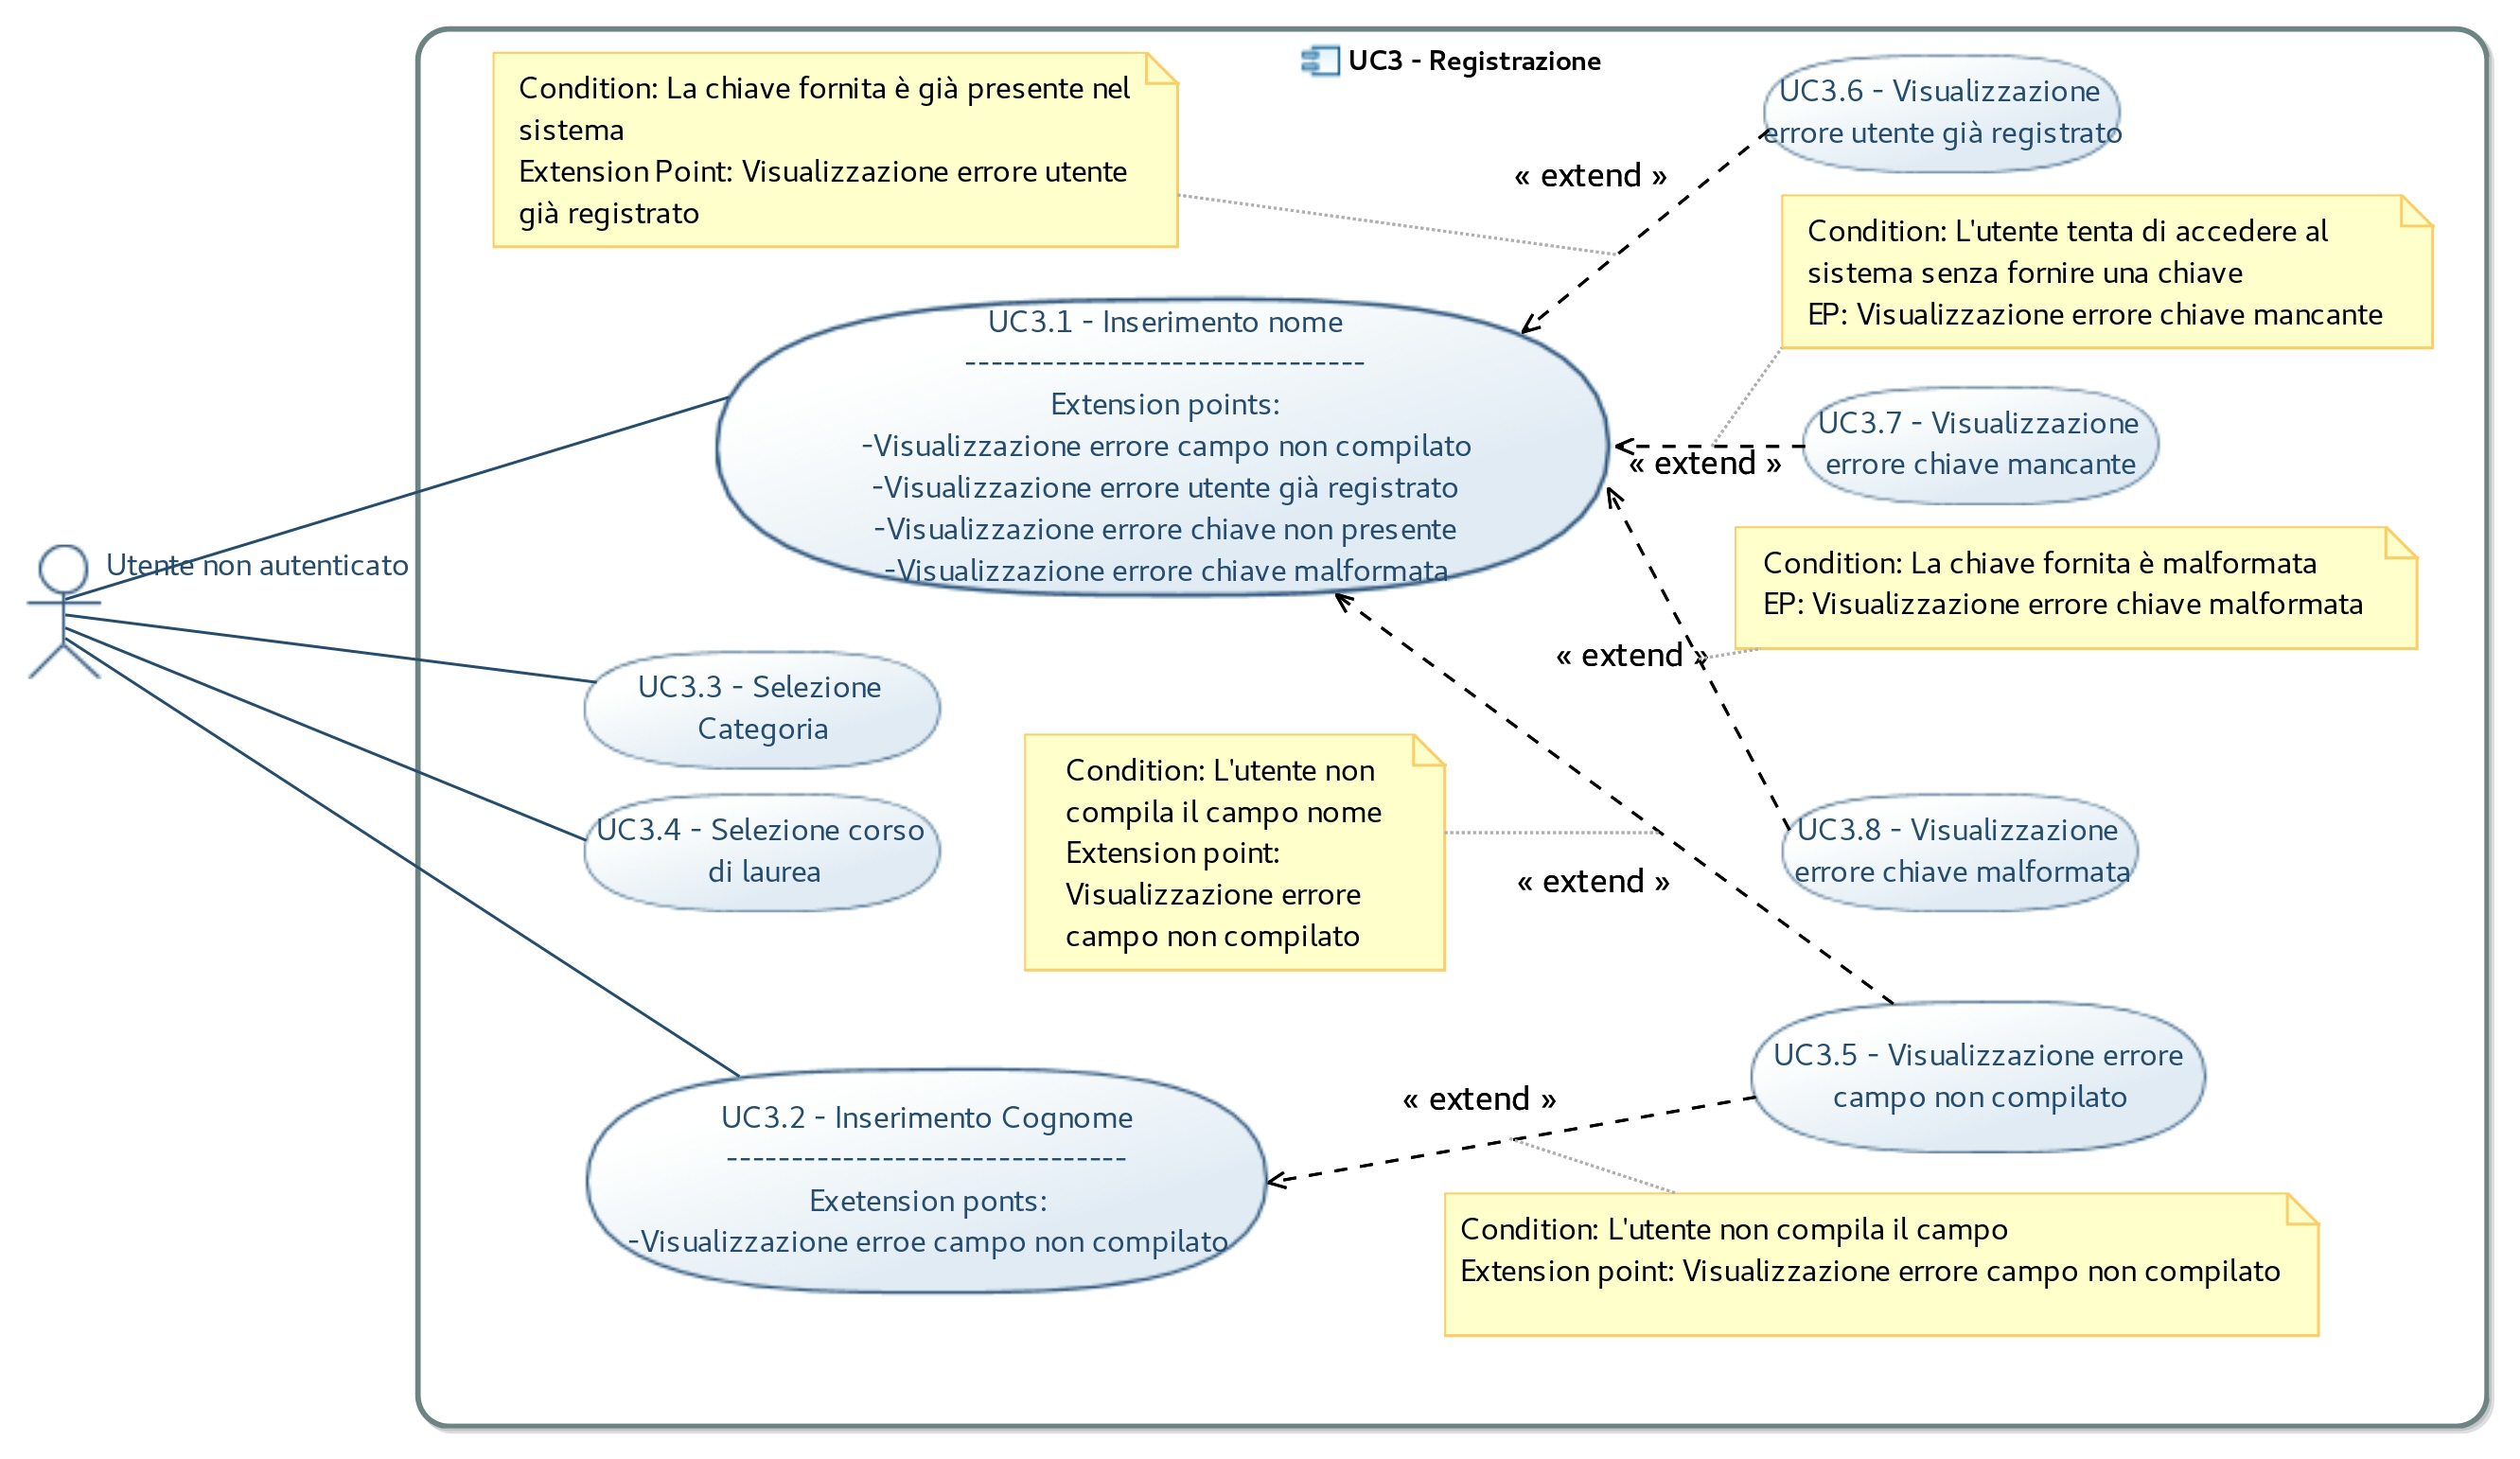
\includegraphics[width=1.0\linewidth]{UC3.jpg}
	\caption{UC3 - Registrazione}
	\label{fig:UC3 - Registrazione}
\end{figure}


\subsection{UC3.1 - Inserimento nome}
\begin{itemize}
	\item \textbf{Attori Primari:} utente non autenticato;
	\item \textbf{Scopo e Descrizione} il sistema \citGloss{verifica} la validità della chiave ed offre l'interfaccia per inserire il nome dell'utente;
	\item \textbf{Scenario principale:} l'utente fornisce tramite un dispositivo di input il suo nome;
	\item \textbf{Estensioni:}
		\begin{enumerate}
			\item se l'utente non ha un chiave viene avvisato tramite un messaggio d'errore [UC3.7];
			\item se l'utente non ha una chiave dal formato non corretto viene avvisato tramite messaggio d'errore [UC3.8];
			\item se la chiave fornita dall'utente è già presente nel sistema l'utente viene avvisato tramite un messaggio d'errore [UC3.6];
			\item se l'utente non compila il campo viene avvisato con un messaggio d'errore [UC3.5].
		\end{enumerate}
	\item \textbf{Precondizione:} l'utente vuole inserire il proprio nome per poter proseguire con la procedura di registrazione;
	\item \textbf{Postcondizione:} l'utente ha inserito il proprio nome nel campo fornito dal sistema e la validità della sua chiave è stata controllata;
\end{itemize}	
\subsection{UC3.2 - Inserimento cognome}
\begin{itemize}
	\item \textbf{Attori Primari:} utente non autenticato;
	\item \textbf{Scopo e Descrizione} il sistema offre l'interfaccia per inserire il cognome dell'utente;
	\item \textbf{Scenario principale:} l'utente fornisce tramite un dispositivo di input il suo cognome;
	\item \textbf{Estensioni:}
		\begin{enumerate}
				\item se l'utente non compila il campo viene avvisato dal sistema [UC3.5].
		\end{enumerate}		
	\item \textbf{Precondizione:} l'utente vuole inserire il proprio cognome;
	\item \textbf{Postcondizione:} l'utente ha inserito il suo cognome nel campo fornito dal sistema;
\end{itemize}
\subsection{UC3.3 - Selezione categoria}
\begin{itemize}
	\item \textbf{Attori Primari:} utente non autenticato;
	\item \textbf{Scopo e Descrizione} il sistema offre l'interfaccia per selezionare la categoria di registrazione (studente o professore);
	\item \textbf{Scenario principale:} l'utente seleziona tramite un dispositivo di input la sua categoria;
	\item \textbf{Precondizione:} l'utente vuole inserire la sua categoria di registrazione;
	\item \textbf{Postcondizione:} l'utente ha selezionato la sua categoria nel campo fornito dal sistema, se la categoria scelta è quella del professore l'utente termina la procedura di registrazione;
\end{itemize}
\subsection{UC3.4 - Selezione corso}
\begin{itemize}
	\item \textbf{Attori Primari:} utente non autenticato;
	\item \textbf{Scopo e Descrizione} il sistema offre l'interfaccia per selezionare il \citGloss{corso di laurea} desiderato;
	\item \textbf{Scenario principale:} l'utente seleziona tramite un dispositivo di input il \citGloss{corso di laurea} scelto;
	\item \textbf{Precondizione:} l'utente ha selezionato la registrazione come studente, il sistema offre un campo per la selezione del \citGloss{corso di laurea} e rimane in attesa dell'input;
	\item \textbf{Postcondizione:} l'utente ha selezionato il suo \citGloss{corso di laurea} nel campo fornito dal sistema e termina la procedura di registrazione;
\end{itemize}
\subsection{UC3.5 - Visualizzazione errore campo non compilato}
\begin{itemize}
	\item \textbf{Attori Primari:} utente non autenticato;
	\item \textbf{Scopo e Descrizione} il sistema avvisa l'utente che non ha compilato il campo selezionato;
	\item \textbf{Scenario principale:} il sistema mostra un messaggio d'errore all'utente che indica la mancata compilazione del campo selezionato;
	\item \textbf{Precondizione:} l'utente non compila il campo selezionato;
	\item \textbf{Postcondizione:} l'utente è consapevole di non aver compilato il campo selezionato;
\end{itemize}
\subsection{UC3.6 - Visualizzazione errore utente già registrato}
\begin{itemize}
	\item \textbf{Attori Primari:} utente non autenticato;
	\item \textbf{Scopo e Descrizione} il sistema avvisa l'utente che la sua chiave è già presente nel sistema e che non può procedere alla registrazione;
	\item \textbf{Scenario principale:} il sistema mostra un messaggio d'errore all'utente che indica che sta tentando di effettuare una registrazione utilizzando una chiave già presente nell'università;
	\item \textbf{Precondizione:} l'utente tenta di registrarsi utilizzando una chiave già registrata;
	\item \textbf{Postcondizione:} l'utente è consapevole di star utilizzando una chiave che corrisponde ad un account precedentemente registrato nel sistema;
\end{itemize}
\subsection{UC3.7 - Visualizzazione errore chiave non presente}
\begin{itemize}
	\item \textbf{Attori Primari:} utente non autenticato;
	\item \textbf{Scopo e Descrizione} il sistema avvisa l'utente che non ha fornito una chiave e quindi non può procedere alla registrazione;
	\item \textbf{Scenario principale:} il sistema mostra un messaggio d'errore all'utente indicandogli l'assenza della chiave;
	\item \textbf{Precondizione:} l'utente tenta di registrarsi senza fornire una chiave;
	\item \textbf{Postcondizione:} l'utente è consapevole di non possedere una chiave;
\end{itemize}
\subsection{UC3.8 - Visualizzazione errore chiave malformata}
\begin{itemize}
	\item \textbf{Attori Primari:} utente non autenticato;
	\item \textbf{Scopo e Descrizione} il sistema avvisa l'utente che ha fornito una chiave malformata e quindi non può procedere alla registrazione;
	\item \textbf{Scenario principale:} il sistema mostra un messaggio d'errore all'utente indicandogli che la sua chiave è malformata;
	\item \textbf{Precondizione:} l'utente tenta di registrarsi fornendo una chiave malformata;
	\item \textbf{Postcondizione:} l'utente è consapevole di possedere una chiave malformata;
\end{itemize}
\subsection{UC4 - Logout}
\begin{itemize}
	\item \textbf{Attori primari:} utente Autenticato;
	\item \textbf{Scopo e descrizione:} l'utente desidera effettuare il logout dal sistema e gli vengono fornite le istruzioni per effettuarlo, in quanto per completare l'operazione l'utente deve interagire direttamente con il plugin \citGloss{MetaMask};
	\item \textbf{Scenario principale:} l'utente autenticato richiede il logout dal sistema;
	\item \textbf{Precondizione:} l'utente è autenticato e vuole effettuare il logout;
	\item \textbf{Postcondizione:} l'utente è informato riguardo alla modalità di logout dal sistema.
\end{itemize}

\subsection{UC5 - Amministrazione}
\begin{itemize}
	\item \textbf{Attori primari:} amministratore;
	\item \textbf{Attori secondari:} \citGloss{MetaMask};
	\item \textbf{Scopo e descrizione:} l'amministratore è nella sua area personale e ottiene una lista di azioni da compiere;
	\item \textbf{Scenario principale:} l'utente visualizza le azioni che può compiere e ne sceglie una; 
	\item \textbf{Precondizione:} l'utente è riconosciuto dal sistema come amministratore e vuole eseguire delle operazioni; 
	\item \textbf{Postcondizione:} l'utente è a conoscenza delle azioni che può eseguire e ne ha scelta una.
\end{itemize}

\begin{figure}[H]
	\centering
	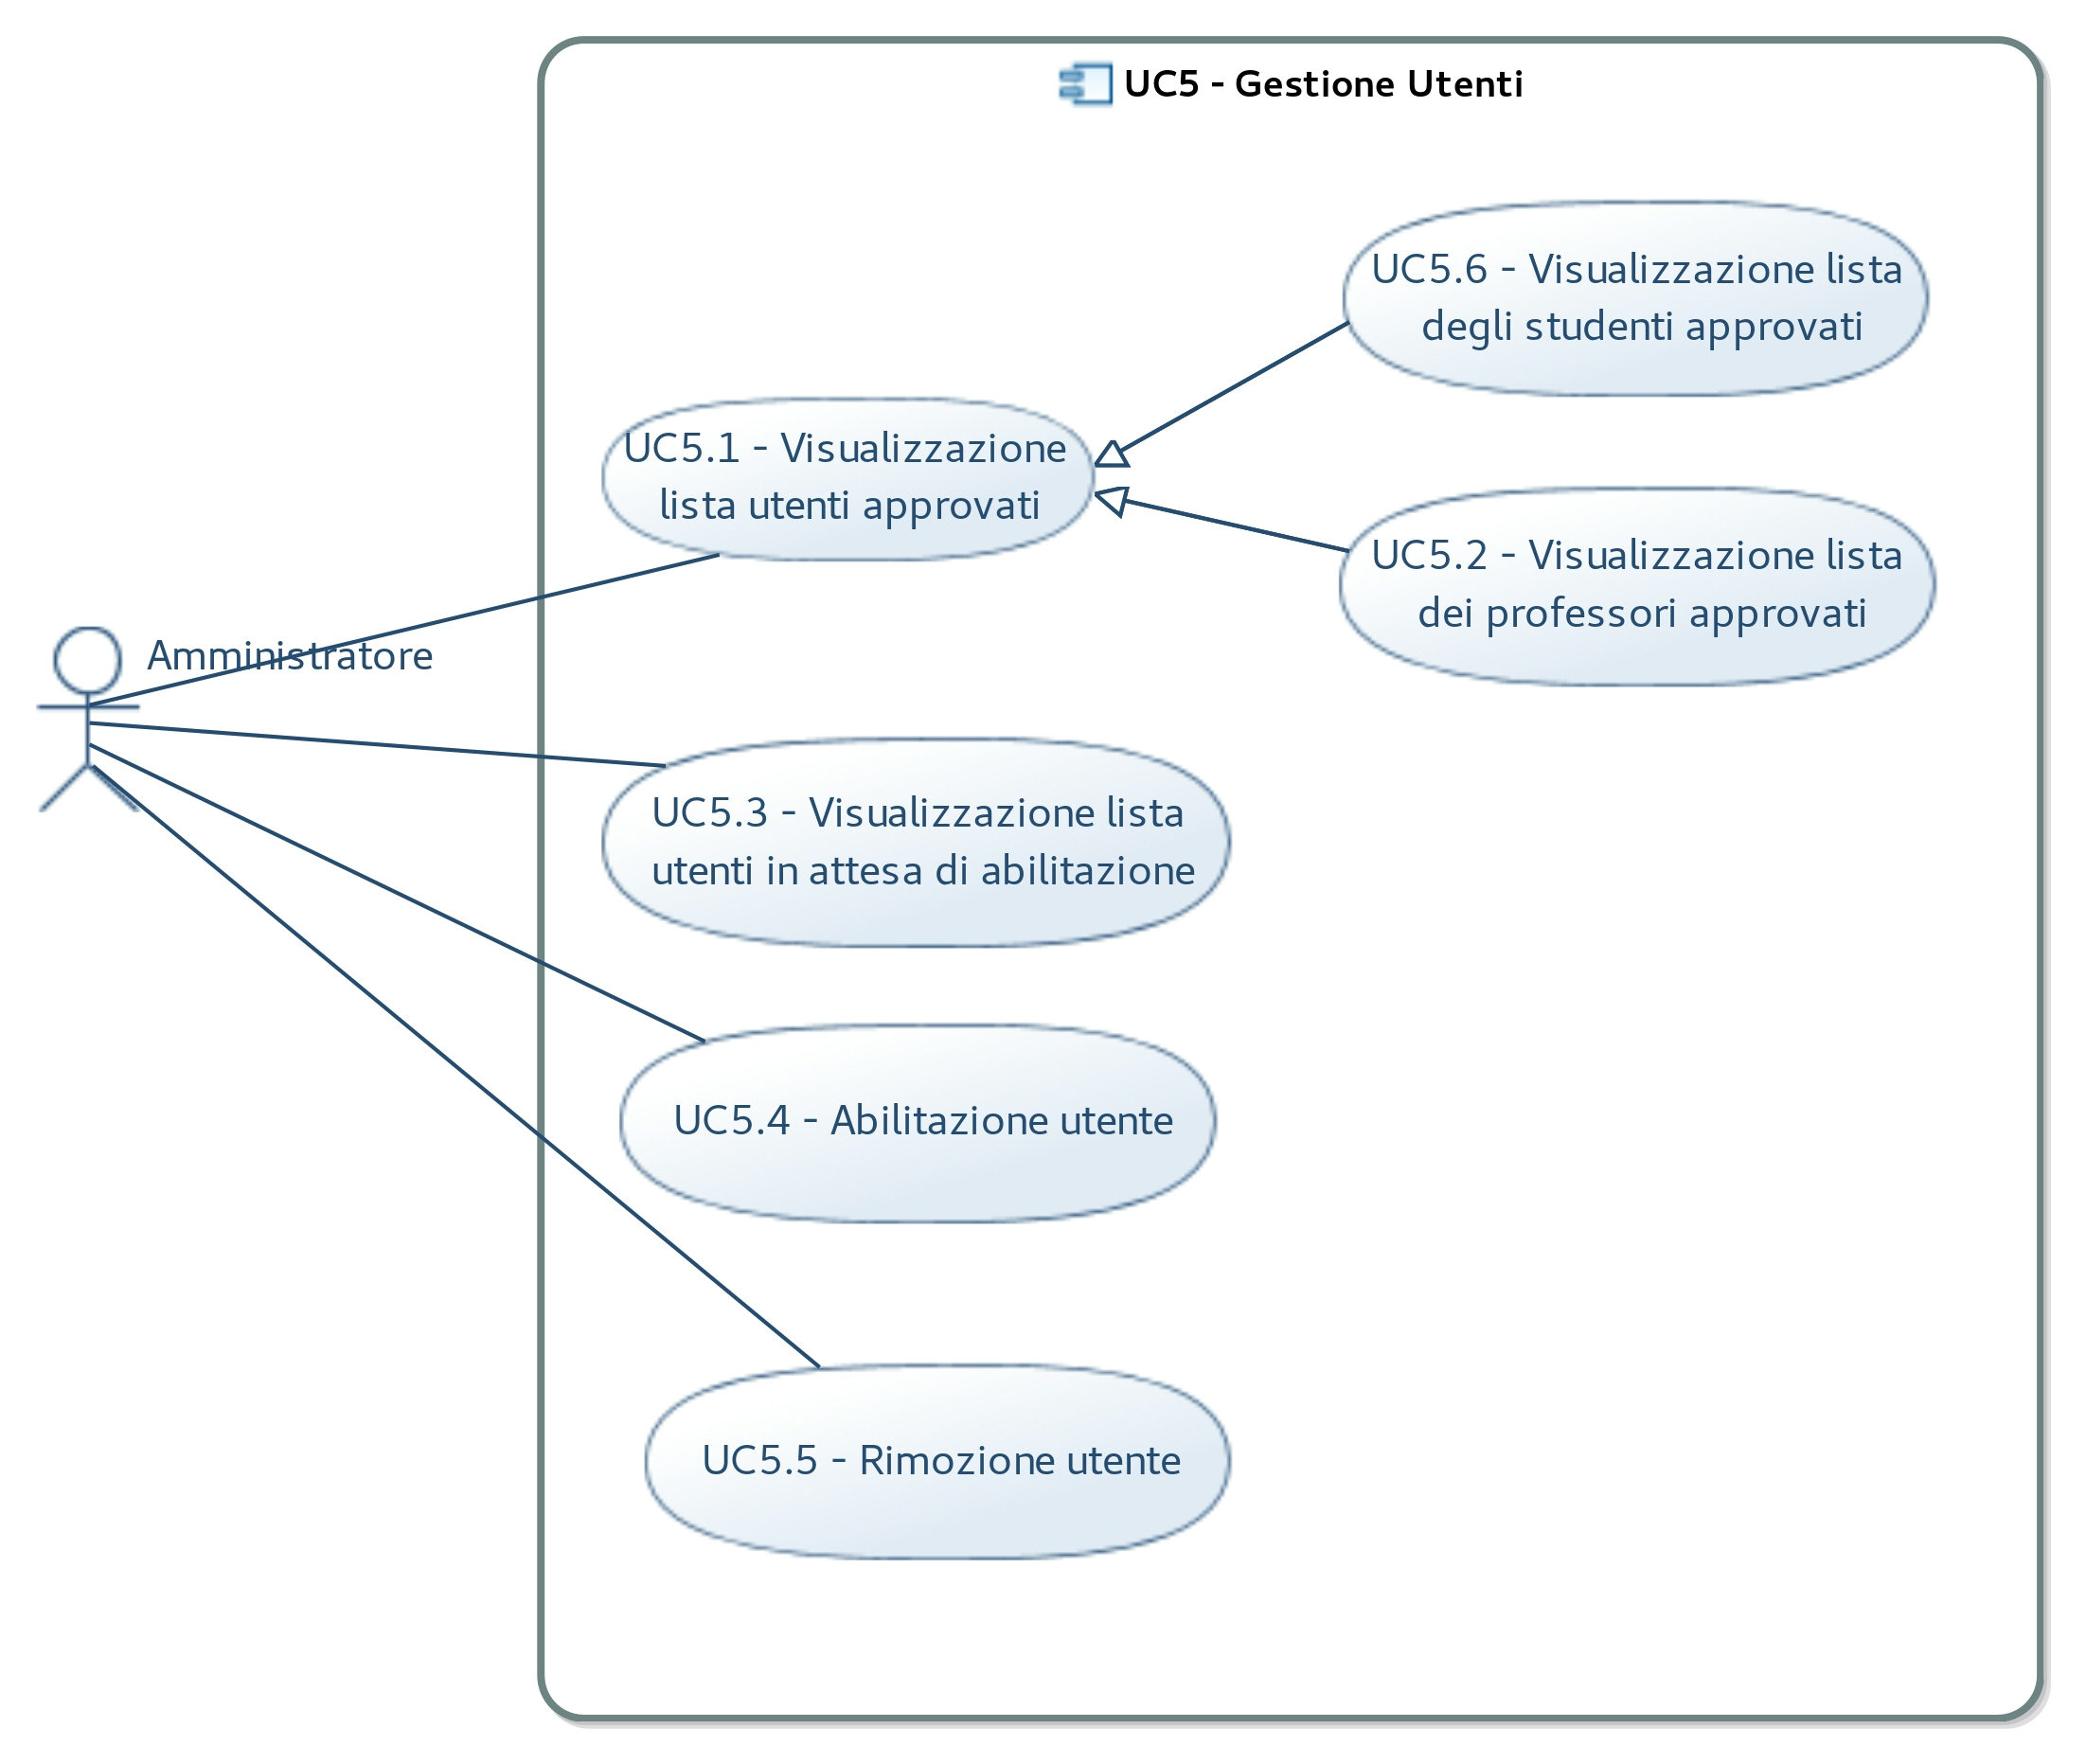
\includegraphics[width=1.0\linewidth]{UC5.jpg}
	\caption{UC5 - Amministrazione}
	\label{fig:UC5 - Amministrazione}
\end{figure}

\subsection{UC5.1 - Gestione Utenti}
\begin{itemize}
	\item \textbf{Attori primari:} amministratore;
	\item \textbf{Scopo e descrizione:} l'amministratore è in grado di eseguire operazioni sugli studenti all'interno dell'ateneo;
	\item \textbf{Scenario principale:} l'amministratore visualizza una lista di operazioni eseguibili sugli studenti e sceglie quale fare;
	\item \textbf{Precondizione:} l'amministratore ha scelto di gestire gli studenti; 
	\item \textbf{Postcondizione:}l'amministratore è a conoscenza delle operazioni che può eseguire sugli studenti e decide di effettuarne una.
\end{itemize}

\begin{figure}[H]
	\centering
	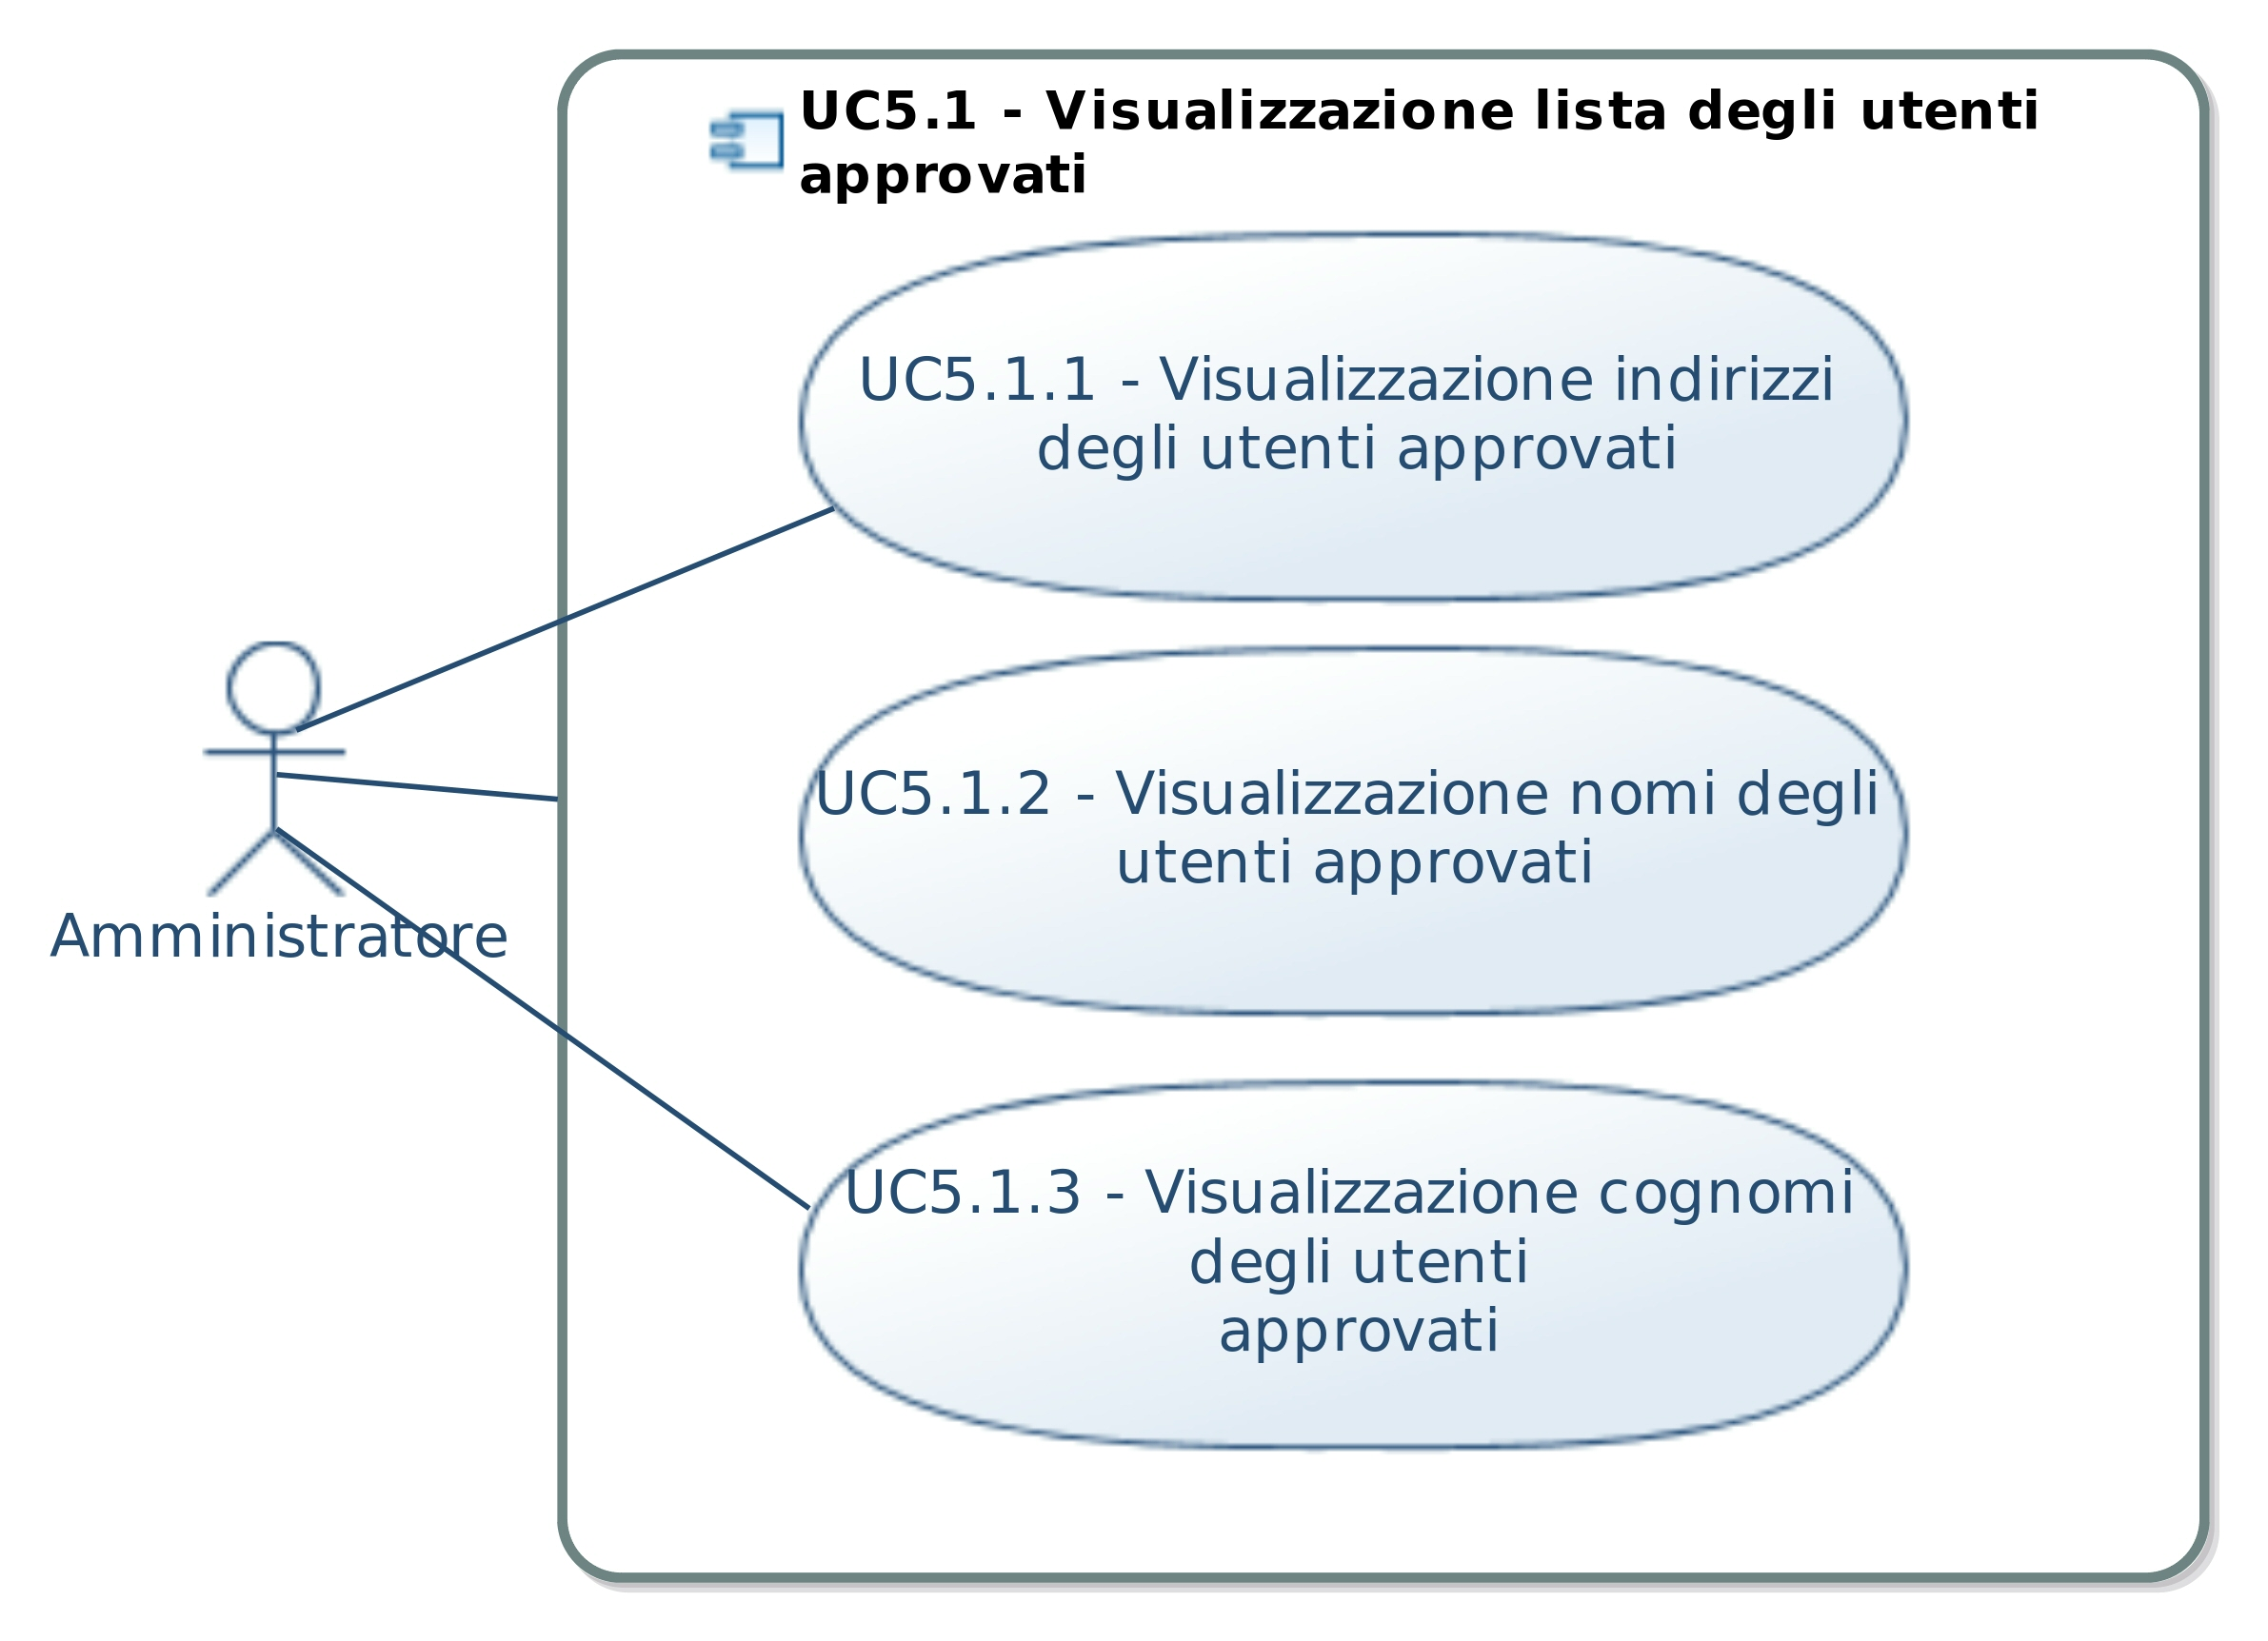
\includegraphics[width=1.0\linewidth]{UC5_1.jpg}
	\caption{UC5.1 - Gestione Utenti}
	\label{fig:UC5.1 - Gestione Utenti}
\end{figure}

\subsection{UC5.1.1 - Visualizzazione lista di studenti}
\begin{itemize}
	\item \textbf{Attori primari:} amministratore;
	\item \textbf{Scopo e descrizione:} l'amministratore visualizza una lista di tutti gli studenti registrati nel sistema;
	\item \textbf{Scenario principale:} l'amministratore richiede al sistema una lista di studenti per poterli gestire;
	\item \textbf{Precondizione:} l'amministratore è nell'area di gestione utenti e richiede una lista di tutti gli studenti; 
	\item \textbf{Postcondizione:} l'amministratore ottiene la lista.
\end{itemize}
\subsection{UC5.1.2 - Visualizzazione lista di professori}
\begin{itemize}
	\item \textbf{Attori primari:} amministratore;
	\item \textbf{Scopo e descrizione:} l'amministratore visualizza una lista di tutti i professori registrati nel sistema;
	\item \textbf{Scenario principale:} l'amministratore richiede al sistema una lista di professori per poterli gestire;
	\item \textbf{Precondizione:} l'amministratore è nell'area di gestione utenti e richiede una lista di tutti i professori; 
	\item \textbf{Postcondizione:} l'amministratore ottiene la lista.
\end{itemize}
\subsection{UC5.1.3 - Visualizzazione lista di utenti in attesa di abilitazione}
\begin{itemize}
	\item \textbf{Attori primari:} amministratore;
	\item \textbf{Scopo e descrizione:} l'amministratore visualizza una lista di tutti gli studenti ancora non abilitati;
	\item \textbf{Scenario principale:} l'amministratore richiede al sistema una lista di studenti in attesa di abilitazione per poterli gestire;
	\item \textbf{Precondizione:}l'amministratore è nell'area di gestione studenti e richiede una lista di studenti in attesa di abilitazione; 
	\item \textbf{Postcondizione:} l'amministratore ottiene la lista.
\end{itemize}
\subsection{UC5.1.4 - Abilitazione utente}
\begin{itemize}
	\item \textbf{Attori primari:} amministratore;
	\item \textbf{Scopo e descrizione:} l'amministratore abilita la registrazione di un utente;
	\item \textbf{Scenario principale:}
	\begin{enumerate}
		\item l'amministratore visualizza la lista degli utenti in attesa di abilitazione [UC5.1.3];
		\item l'amministratore lo abilita [UC5.1.4].
	\end{enumerate}
	\item \textbf{Precondizione:} l'amministratore ha richiesto una lista di utenti non abilitati; 
	\item \textbf{Postcondizione:} l'amministratore selezionato viene abilitato e il suo stato viene aggiornato nel sistema.
\end{itemize}
\subsection{UC5.1.5 - Rimozione utente}
\begin{itemize}
	\item \textbf{Attori primari:} amministratore;
	\item \textbf{Scopo e descrizione:} l'amministratore rimuove dal sistema un utente non ancora abilitato o già abilitato;
	\item \textbf{Scenario principale:}
	\begin{enumerate}
		\item l'amministratore visualizza gli utenti abilitati o in attesa di abilitazione e ne seleziona uno [UC5.1.1 o UC5.1.2 o UC5.3];
		\item l'amministratore rimuove l'utente selezionato [UC5.1.5].
	\end{enumerate}
	\item \textbf{Precondizione:} l'amministratore ha richiesto una lista di studenti o professori; 
	\item \textbf{Postcondizione:} l'utente selezionato viene rimosso dal sistema.
\end{itemize}
\subsection{UC5.2 - Gestione anni accademici}
\begin{itemize}
	\item \textbf{Attori primari:} amministratore;
	\item \textbf{Scopo e descrizione:} l'amministratore è in grado di eseguire operazioni sugli anni accademici dell'ateneo;
	\item \textbf{Scenario principale:} l'amministratore visualizza una lista di operazioni eseguibili sugli anni accademici e ne sceglie una;
	\item \textbf{Precondizione:} l'amministratore ha scelto di gestire gli anni accademeici; 
	\item \textbf{Postcondizione:} l'amministratore è a conoscenza delle possibili operazioni da eseguire sugli anni accademici e ne ha scelta una.
\end{itemize}

\begin{figure}[H]
	\centering
	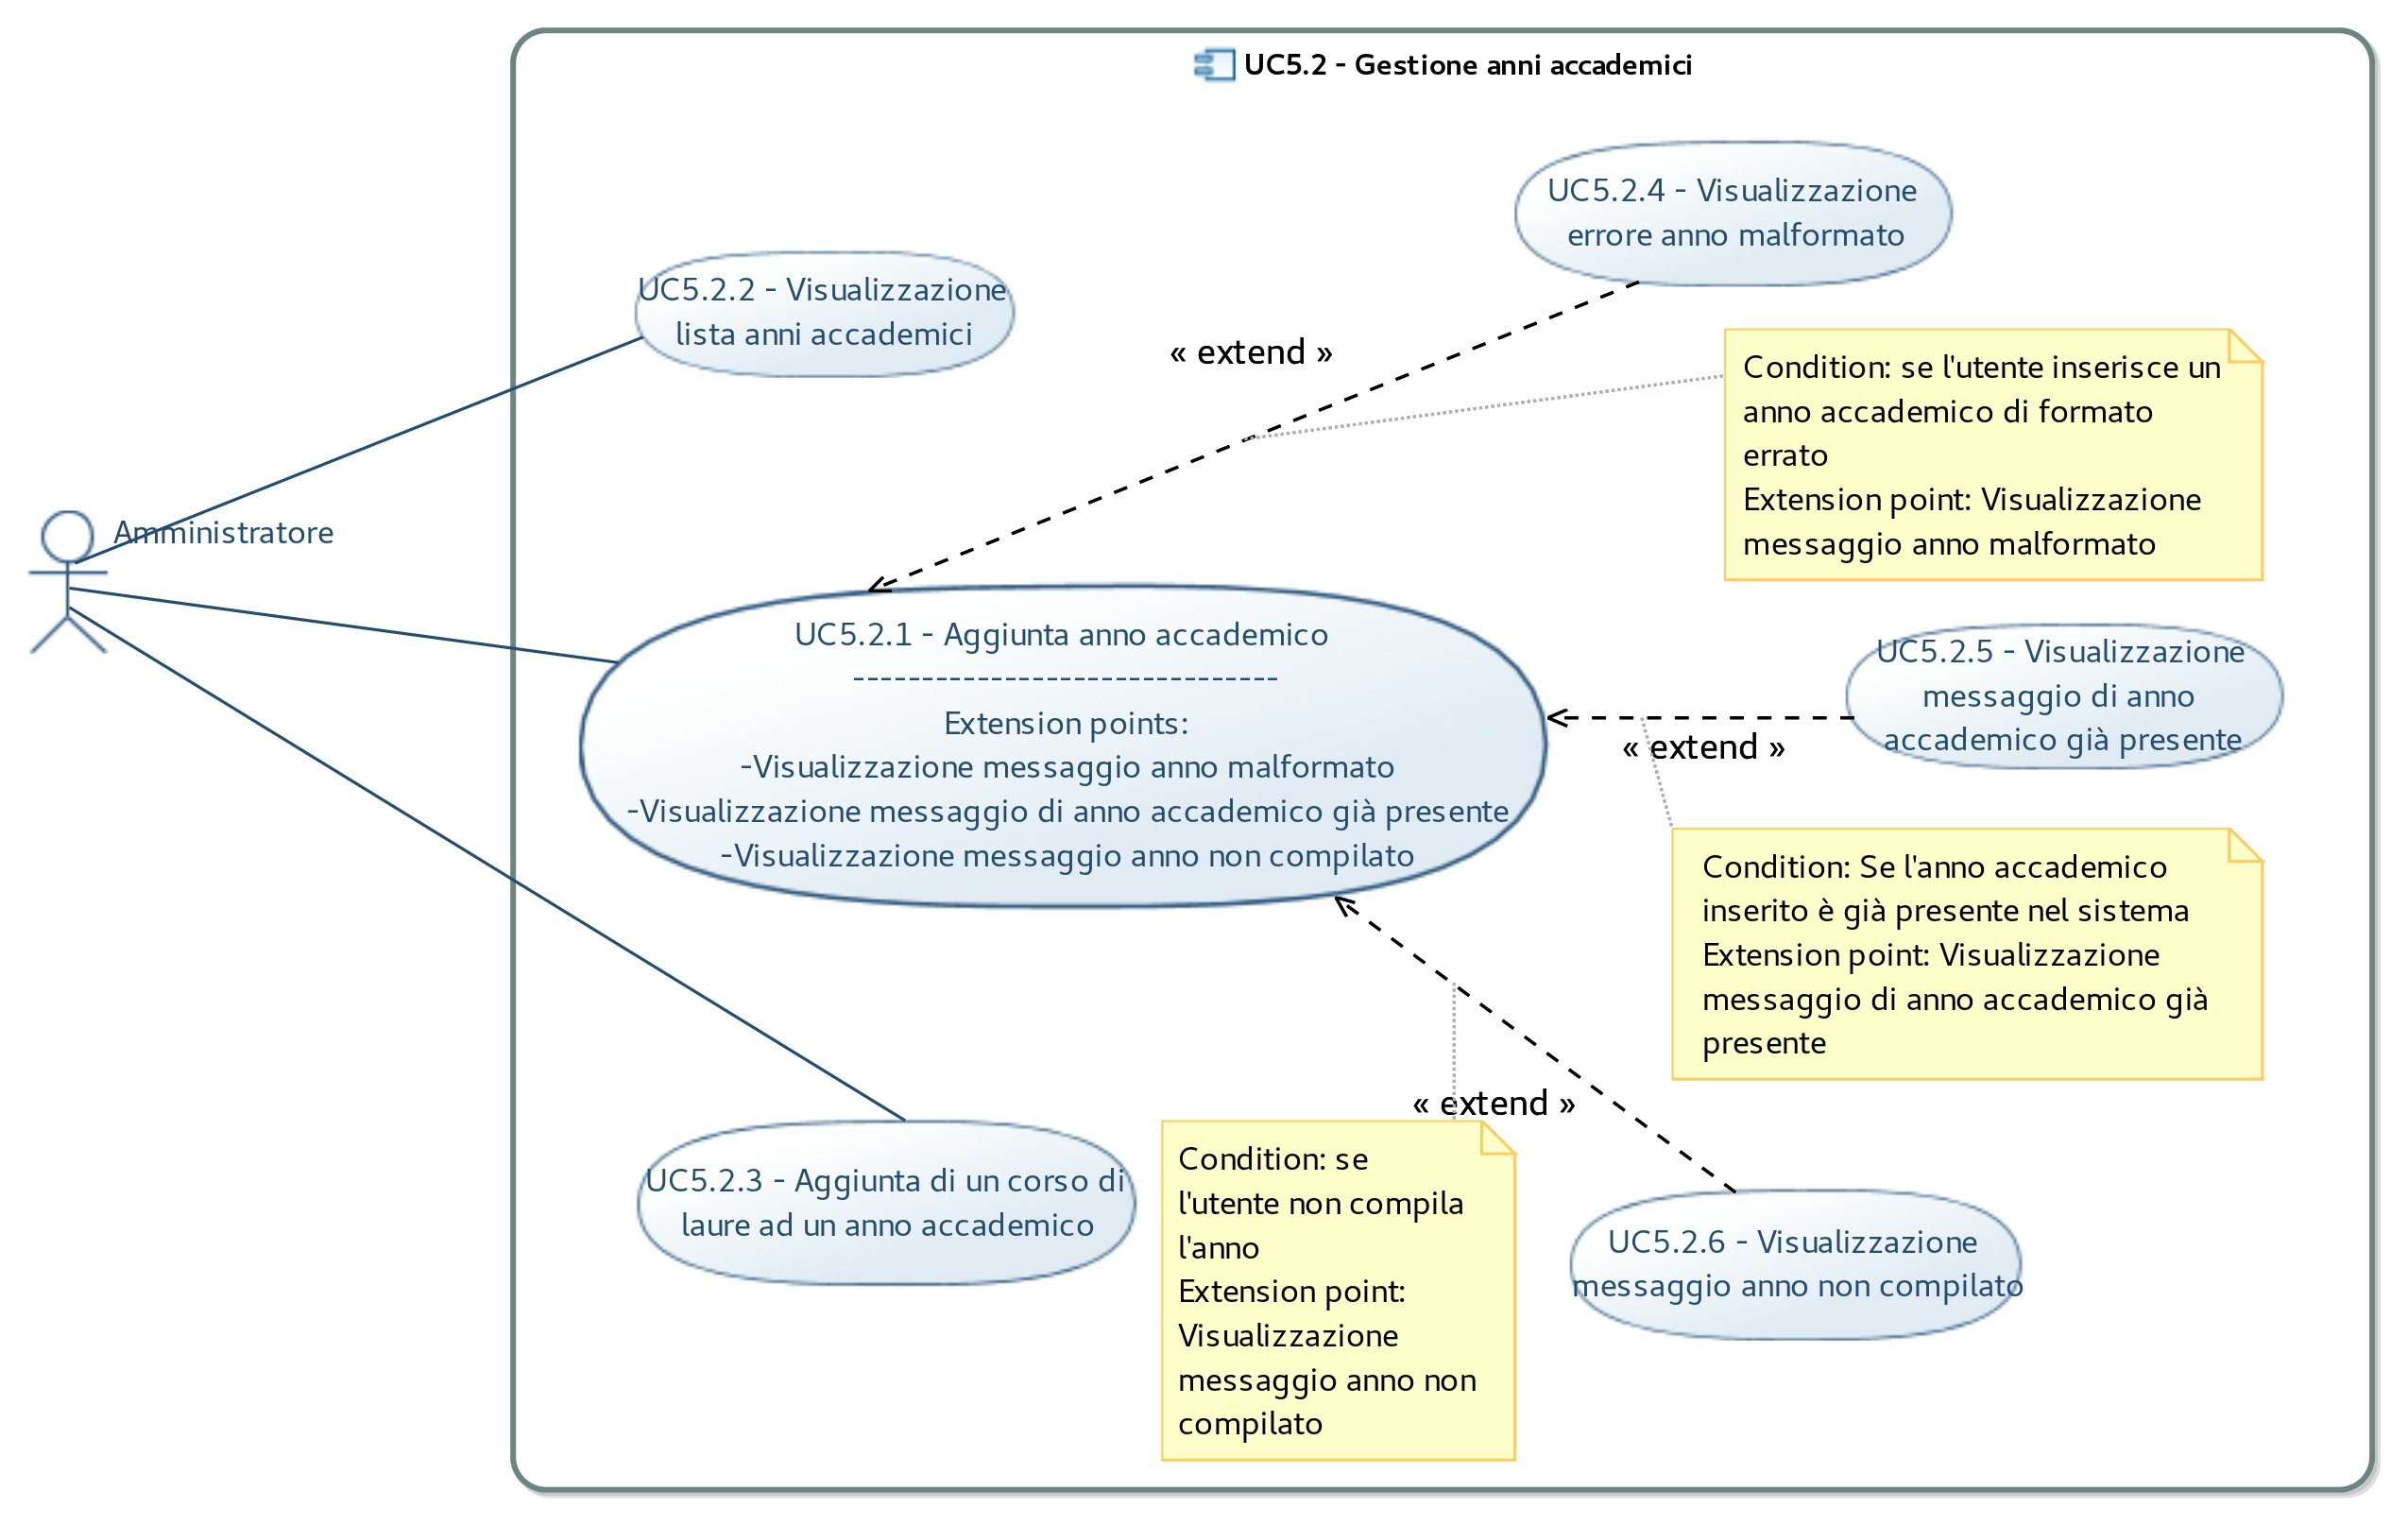
\includegraphics[width=1.0\linewidth]{UC5_2.jpg}
	\caption{UC5.2 - Gestione Anni Accademici}
	\label{fig:UC5.2 - Gestione Anni Accademici}
\end{figure}

\subsection{UC5.2.1 - Aggiunta anno accademico}
\begin{itemize}
	\item \textbf{Attori primari:} amministratore;
	\item \textbf{Scopo e descrizione:} l'amministratore aggiunge un \citGloss{anno accademico} nel sistema;
	\item \textbf{Scenario principale:} l'amministratore inserisce il numero dell'anno da aggiungere in un campo fornito dal sistema;
	\item \textbf{Estensioni:}
	\begin{enumerate}
		\item se l'amministratore inserisce un'anno non numerico viene mostrato un messaggio d'errore relativo alla malformazione dell'anno [UC5.1.4];
		\item se l'amministratore inserisce un'anno già presente nel sistema viene mostrato un messaggio d'errore relativo alla non univocità dell'anno [UC5.1.5];
		\item se l'amministratore lascia il campo vuoto l'utente viene avvisato con un relativo messaggio d'errore [UC5.1.6].
	\end{enumerate}
	\item \textbf{Precondizione:} l'amministratore ha scelto di aggiungere un \citGloss{anno accademico}; 
	\item \textbf{Postcondizione:} l'\citGloss{anno accademico} creato viene inserito nel sistema.
\end{itemize}
\subsection{UC5.2.2 - Visualizzazione lista di tutti gli anni accademici}
\begin{itemize}
	\item \textbf{Attori primari:} amministratore;
	\item \textbf{Scopo e descrizione:} l'amministratore visualizza una lista di tutti gli anni accademici presenti nel sistema;
	\item \textbf{Scenario principale:} l'amministratore richiede la lista di tutti gli anni del sistema;
	\item \textbf{Precondizione:} l'amministratore è nell'area di gestione Anni Accademici e vuole ottenere la lista di tutti gli anni presenti nel sistema; 
	\item \textbf{Postcondizione:} l'amministratore ottiene la lista.
\end{itemize}
\subsection{UC5.2.3 - Aggiunta di un corso di laurea ad un anno accademico}
\begin{itemize}
	\item \textbf{Attori primari:} amministratore;
	\item \textbf{Scopo e descrizione:} l'amministratore aggiunge un corso di laurea già presente nel sistema all'interno dell'\citGloss{anno accademico};
	\item \textbf{Scenario principale:}
	\begin{enumerate}
		\item l'amministratore visualizza la lista degli anni accademici e identifica quello di suo interesse [UC5.2.2];
		\item l'amministratore ottiene una lista dei corsi di laurea [UC 5.3.3];
		\item l'amministratore seleziona il \citGloss{corso di laurea} e lo inserisce all'interno dell'\citGloss{anno accademico} desiderato [5.2.3].
	\end{enumerate}
	\item \textbf{Precondizione:} l'amministratore vuole aggiungere un corso di laurea all'\citGloss{anno accademico} è ha ottenuto una lista degli anni accademici presenti nel sistema; 
	\item \textbf{Postcondizione:} il corso di laurea è stato correlato con l'\citGloss{anno accademico} e il loro stato è stato aggiornato nel sistema.
\end{itemize}
\subsection{UC5.2.4 - Visualizzazione messaggio anno malformato}
\begin{itemize}
	\item \textbf{Attori primari:} amministratore;
	\item \textbf{Scopo e descrizione:} l'amministratore visualizza un messaggio che lo informa che l'anno inserito non è numerico;
	\item \textbf{Scenario principale:} il sistema mostra all'amministratore un messaggio d'errore relativo alla malformazione dell'anno inserito;
	\item \textbf{Precondizione:} l'amministratore prova a creare un nuovo \citGloss{anno accademico} inserendo un anno non numerico; 
	\item \textbf{Postcondizione:} l'amministratore è consapevole di aver provato ad inserire un anno non numerico.
\end{itemize}
\subsection{UC5.2.5 - Visualizzazione messaggio di anno accademico già presente}
\begin{itemize}
	\item \textbf{Attori primari:} amministratore;
	\item \textbf{Scopo e descrizione:} l'amministratore visualizza un messaggio che indica che un \citGloss{anno accademico} come quello inserito è già presente nel sistema;
	\item \textbf{Scenario principale:} il sistema mostra all'amministratore un messaggio d'errore relativo alla non univocità dell'\citGloss{anno accademico} inserito;
	\item \textbf{Precondizione:} l'amministratore tenta di inserire un \citGloss{anno accademico} già presente nel sistema; 
	\item \textbf{Postcondizione:} l'amministratore è consapevole di aver provato ad inserire un \citGloss{anno accademico} già presente nel sistema.
\end{itemize}
\subsection{UC5.2.6 - Visualizzazione messaggio anno non compilato}
\begin{itemize}
	\item \textbf{Attori primari:} amministratore;
	\item \textbf{Scopo e descrizione:} l'amministratore visualizza un messaggio che lo avvisa aver lasciato vuoto il campo dell'\citGloss{anno accademico};
	\item \textbf{Scenario principale:} il sistema mostra un messaggio d'errore relativo alla non compilazione dell'\citGloss{anno accademico};
	\item \textbf{Precondizione:} l'amministratore tenta di inserire un \citGloss{anno accademico} vuoto; 
	\item \textbf{Postcondizione:} l'amministratore è consapevole di aver provato ad inserire un \citGloss{anno accademico} vuoto.
\end{itemize}
\subsection{UC5.3 - Gestione corsi di laurea}
\begin{itemize}
	\item \textbf{Attori primari:} amministratore;
	\item \textbf{Scopo e descrizione:} l'amministratore è in grado di eseguire operazioni sui corsi di laurea;
	\item \textbf{Scenario principale:} l'amministratore visualizza una lista di operazioni eseguibili sui corsi di laurea e ne sceglie una;
	\item \textbf{Precondizione:} l'utente ha scelto di gestire i corsi di laurea; 
	\item \textbf{Postcondizione:} l'utente è a conoscenza delle possibili operazioni da eseguire sui corsi di laurea e ne ha scelta una.
\end{itemize}

\begin{figure}[H]
	\centering
	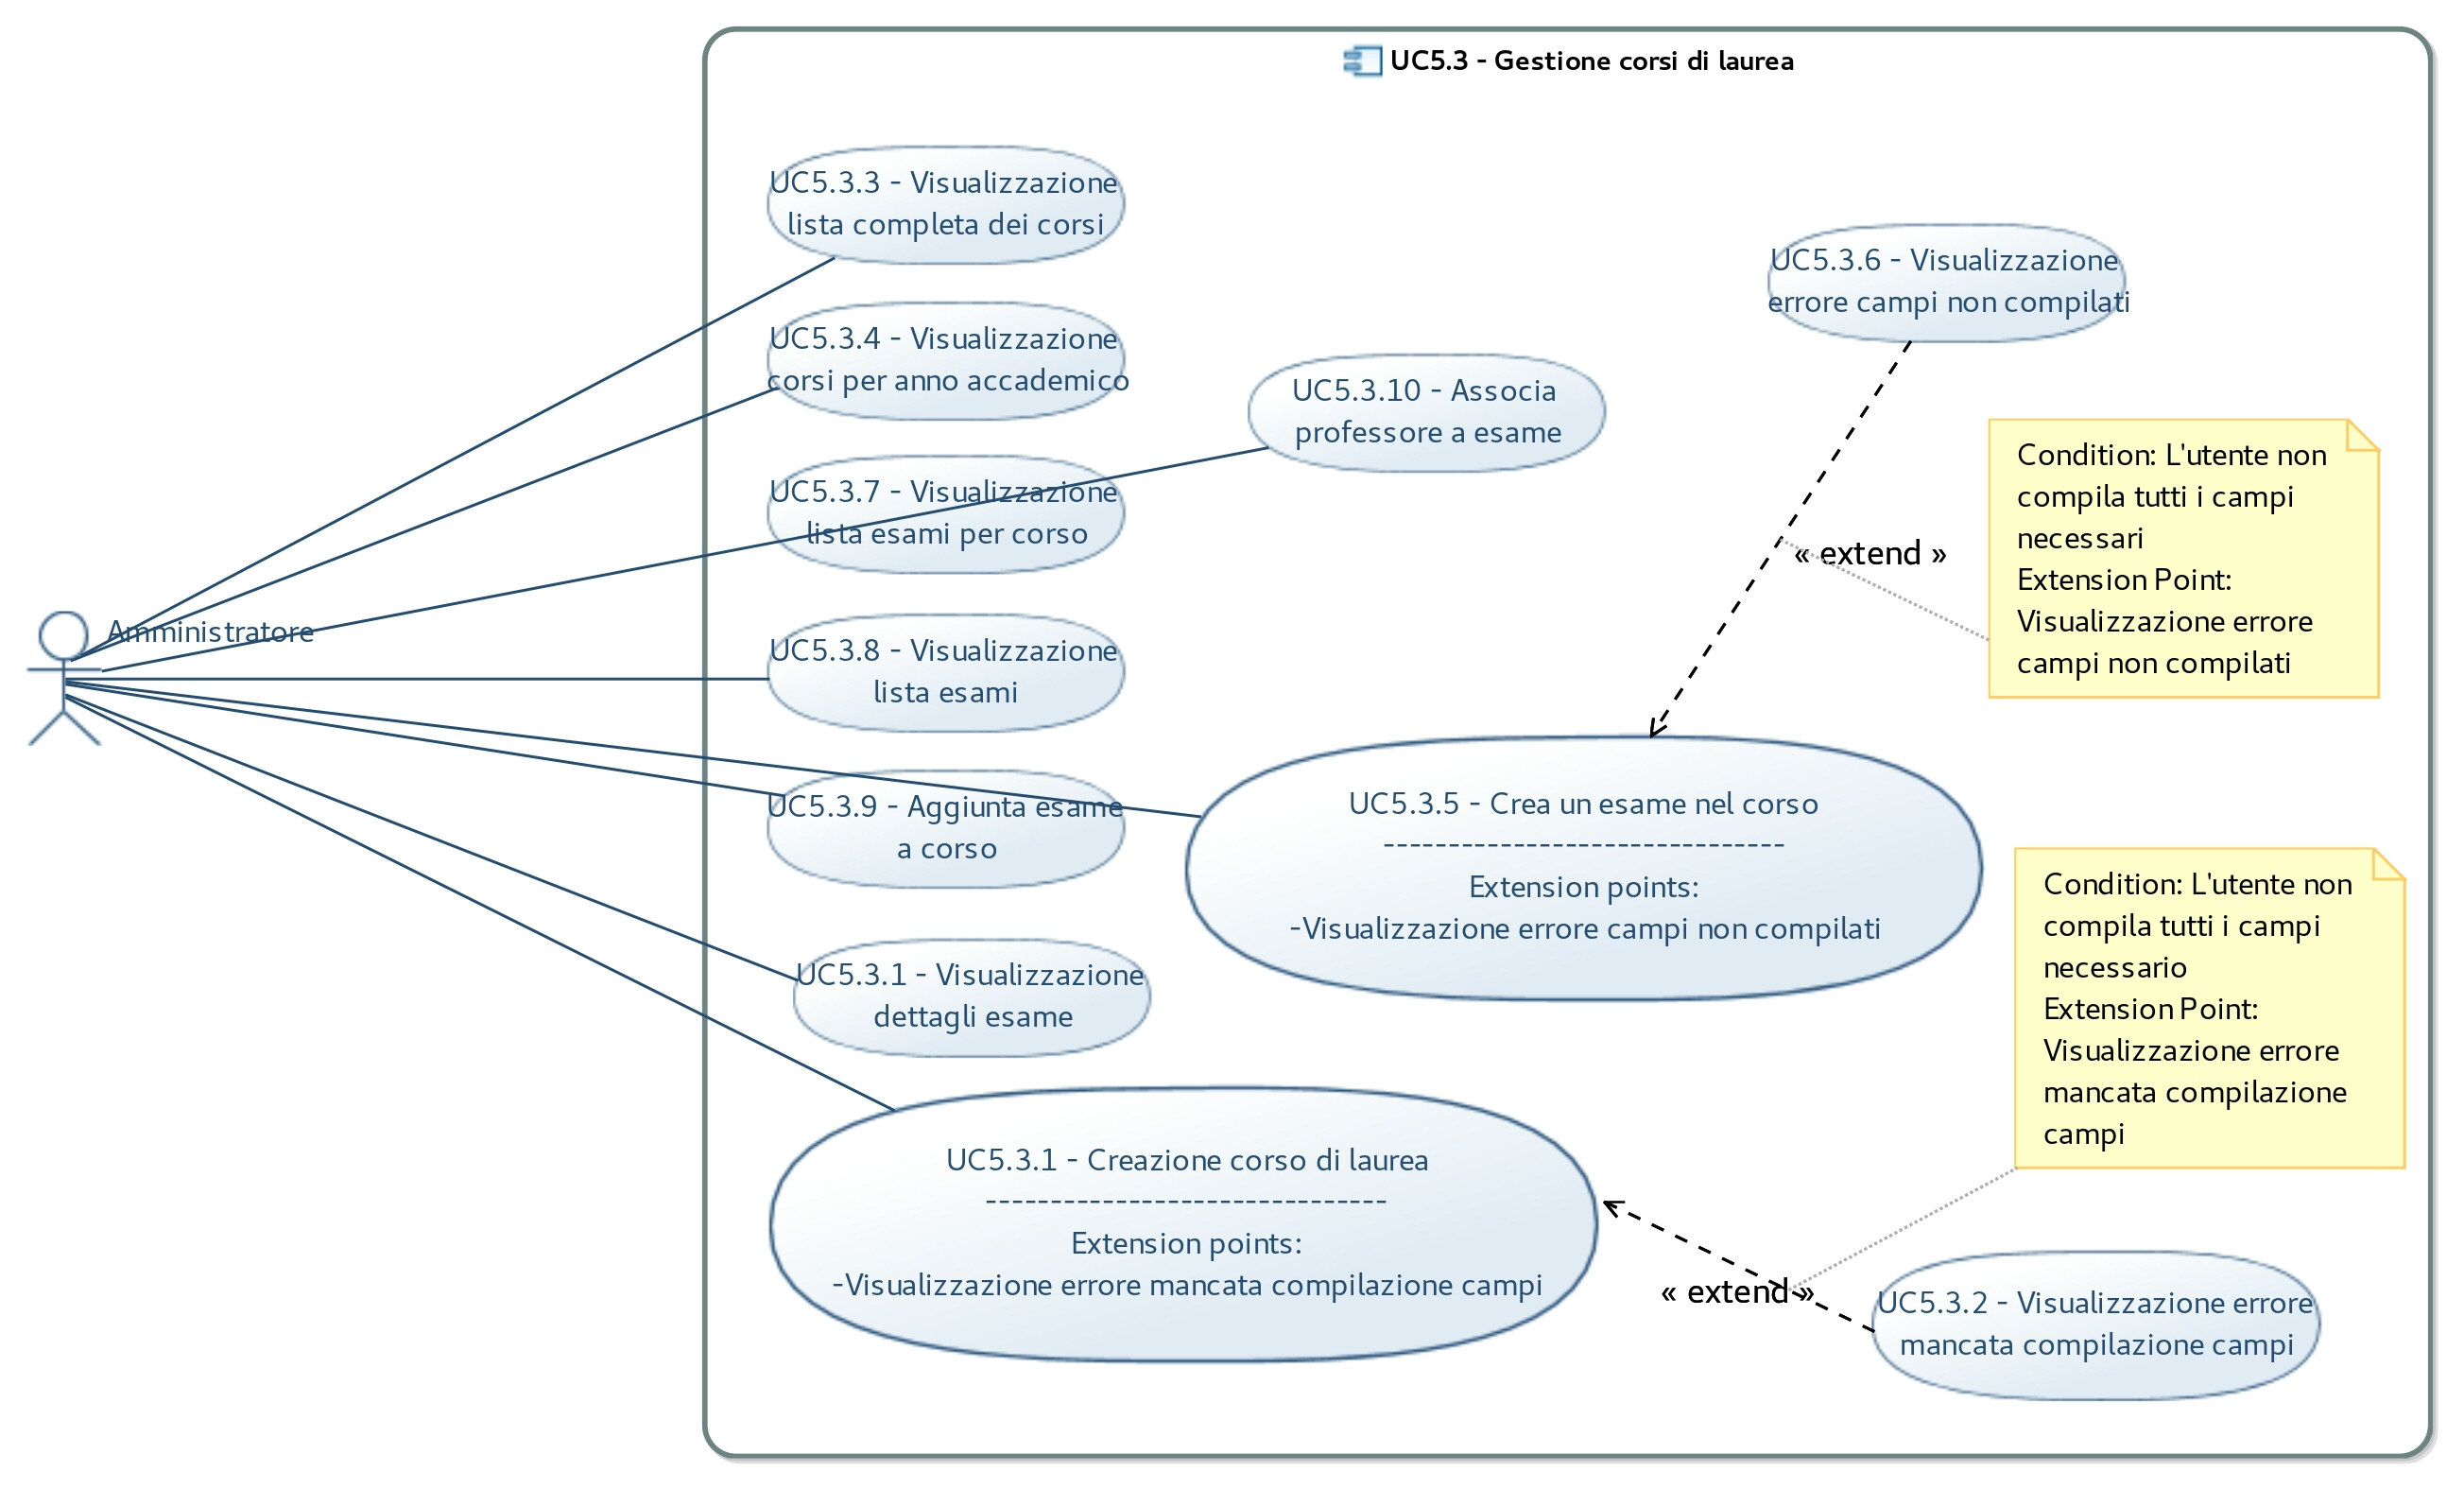
\includegraphics[width=1.0\linewidth]{UC5_3.jpg}
	\caption{UC5.3 - Gestione Corsi di laurea}
	\label{fig:UC5.3 - Gestione Corsi di laurea}
\end{figure}

\subsection{UC5.3.1 - Creazione corso di laurea}
\begin{itemize}
	\item \textbf{Attori primari:} amministratore;
	\item \textbf{Scopo e descrizione:} l'amministratore crea un nuovo corso di laurea associato ad un \citGloss{anno accademico};
	\item \textbf{Scenario principale:}
		\begin{enumerate}
			\item l'amministratore ottiene una lista degli anni accademici e seleziona quello di suo interesse [UC5.2.2];
			\item l'amministratore inserisce di dati relativi al \citGloss{corso di laurea} [5.3.1].
		\end{enumerate}
	\item \textbf{Estensioni:}
		\begin{enumerate}
			\item se l'amministratore non inserisce tutti i campi viene avvisato dal sistema [UC5.3.2].
		\end{enumerate}
	\item \textbf{Precondizione:} l'amministratore vuole inserire un nuovo corso di laurea associato ad un \citGloss{anno accademico}; 
	\item \textbf{Postcondizione:} il \citGloss{corso di laurea} è stato creato ed inserito nel sistema.
\end{itemize}
\subsection{UC5.3.2 - Visualizzazione errore mancata compilazione campi}
\begin{itemize}
	\item \textbf{Attori primari:} amministratore;
	\item \textbf{Scopo e descrizione:} viene mostrato un messaggio d'errore per avvisare l'amministratore che non ha compilato i campi necessari;
	\item \textbf{Scenario principale:} il sistema mostra all'amministratore che non ha compilato tutti i campi;
	\item \textbf{Precondizione:} l'amministratore ha tentato di creare un \citGloss{corso di laurea} senza compilare tutti i campi; 
	\item \textbf{Postcondizione:} l'amministratore è consapevole di non aver inserito tutti i campi necessari.
\end{itemize}\subsection{UC5.3.3 - Visualizzazione lista completa dei corsi}
\begin{itemize}
	\item \textbf{Attori primari:} amministratore;
	\item \textbf{Scopo e descrizione:} vengono mostrati tutti i corsi di laurea presenti nel sistema;
	\item \textbf{Scenario principale:} l'amministratore visualizza tutti i corsi di laurea presenti nel sistema;
	\item \textbf{Precondizione:} l'amministratore ha richiesto la visualizzazione di tutti i corsi di laurea; 
	\item \textbf{Postcondizione:} l'amministratore ottiene la lista.
\end{itemize}
\subsection{UC5.3.4 - Visualizzazione lista corsi di laurea per anno accademico}
\begin{itemize}
	\item \textbf{Attori primari:} amministratore;
	\item \textbf{Scopo e descrizione:} vengono visualizzati i corsi di laurea relativi ad un determinato \citGloss{anno accademico};
	\item \textbf{Scenario principale:}
	\begin{enumerate}
		\item l'amministratore ottiene una lista degli anni accademici e seleziona quello di suo interesse [UC5.2.2];
		\item il sistema mostra la lista di corsi di laurea associati all'\citGloss{anno accademico} [UC5.3.4].
	\end{enumerate};
	\item \textbf{Precondizione:} l'amministratore ha visualizzato una lista di anni accademici [UC5.2.2] e vuole visualizzare i corsi di laurea all'interno di uno di essi; 
	\item \textbf{Postcondizione:} l'amministratore ottiene la lista desiderata.
\end{itemize}
\subsection{UC5.3.5 - Crea un esame nel corso}
\begin{itemize}
	\item \textbf{Attori primari:} amministratore;
	\item \textbf{Scopo e descrizione:} l'amministratore crea ed assegna un esame all'interno di un \citGloss{corso di laurea};
	\item \textbf{Scenario principale:} l'amministratore inserisce i dati necessari per la creazione dell'esame;
	\item \textbf{Estensioni:}
	\begin{enumerate}
		\item se l'amministratore non compila tutti i campi viene visualizzato un messaggio d'errore [UC5.3.4].
	\end{enumerate}
	\item \textbf{Precondizione:} l'amministratore ha ottenuto una lista di corsi di laurea per \citGloss{anno accademico} [UC5.3.3] e ne ha selezionato uno, volendo creare un esame al su interno; 
	\item \textbf{Postcondizione:} l'esame viene inserito nel sistema e associato al \citGloss{corso di laurea} selezionato.
\end{itemize}
\subsection{UC5.3.6 - Visualizzazione errore campi non compilati nella creazione dell'esame}
\begin{itemize}
	\item \textbf{Attori primari:} amministratore;
	\item \textbf{Scopo e descrizione:} viene mostrato un messaggio d'errore relativo alla mancata compilazione dei campi associati all'esame;
	\item \textbf{Scenario principale:} l'amministratore visualizza il messaggio d'errore;
	\item \textbf{Precondizione:} l'amministratore tenta di creare un esame senza compilare tutti i campi obbligatori; 
	\item \textbf{Postcondizione:} l'amministratore è a conoscenza di non aver compilato tutti i campi necessari.
\end{itemize}
\subsection{UC5.3.7 - Visualizzazione lista esami per corso}
\begin{itemize}
	\item \textbf{Attori primari:} amministratore;
	\item \textbf{Scopo e descrizione:} vengono visualizzati gli esami relativi ad un determinato \citGloss{corso di laurea};
	\item \textbf{Scenario principale:}
	\begin{enumerate}
		\item l'amministratore ottiene una lista dei corsi di laurea e seleziona quello di suo interesse [UC5.3.3 o UC5.3.4];
		\item il sistema mostra la lista di esami associati al corso selezionato
	\end{enumerate};
	\item \textbf{Precondizione:} l'amministratore ha visualizzato una lista di corsi di laurea [UC5.3.3 o UC5.3.4] e vuole visualizzare gli esami all'interno di uno di essi; 
	\item \textbf{Postcondizione:} l'amministratore ottiene la lista desiderata.
\end{itemize}
\subsection{UC5.3.8 - Visualizzazione lista esami}
\begin{itemize}
	\item \textbf{Attori primari:} amministratore;
	\item \textbf{Scopo e descrizione:} vengono visualizzati gli esami all'interno del sistema;
	\item \textbf{Scenario principale:} l'amministratore visualizza la lista di tutti gli esami presenti nel sistema;
	\item \textbf{Precondizione:} l'amministratore vuole vedere tutti gli esami presenti nel sistema; 
	\item \textbf{Postcondizione:} l'amministratore ottiene la lista desiderata.
\end{itemize}
\subsection{UC5.3.9 - Aggiunta esame a corso}
\begin{itemize}
	\item \textbf{Attori primari:} amministratore;
	\item \textbf{Scopo e descrizione:} l'amministratore aggiunge un esame ad un determinato \citGloss{corso di laurea};
	\item \textbf{Scenario principale:}
		\begin{enumerate}
			\item l'amministratore ottiene una lista dei corsi di laurea e seleziona quello di suo interesse [UC5.3.3 o UC5.3.4];
			\item l'amministratore ottiene una lista degli esami [UC5.3.7 o UC5.3.8];
			\item l'amministratore seleziona l'esame e lo inserisce all'interno del corso selezionato [UC5.3.9].
		\end{enumerate}
	\item \textbf{Precondizione:} l'amministratore vuole aggiungere un esame ad un \citGloss{corso di laurea} e ha ottenuto una lista di corsi di laurea presenti nel sistema [UC5.3.3 o UC5.3.4]; 
	\item \textbf{Postcondizione:} l'esame è stato aggiunto al \citGloss{corso di laurea} e il loro stato aggiornato nel sistema.
\end{itemize}
\begin{comment}
subsection{UC5.3.10 - Rimozione esame da un corso}
\begin{itemize}
	\item \textbf{Attori primari:} Amministratore;
	\item \textbf{Scopo e descrizione:} L'amministratore rimuove un esame da un \citGloss{corso di laurea};
	\item \textbf{Scenario principale:}
	\begin{enumerate}
		\item L'utente seleziona l'esame e lo rimuove dal corso selezionato;
	\end{enumerate}
	\item \textbf{Precondizione:}L'utente ha ottenuto una lista di esami associati dal \citGloss{corso di laurea} [UC5.3.7] e ne vuole rimuovere uno dal corso; 
	\item \textbf{Postcondizione:} L'esame è rimosso dal \citGloss{corso di laurea}.
\end{itemize}
\end{comment}
\subsection{UC5.3.10 - Associazione professore a esame}
\begin{itemize}
	\item \textbf{Attori primari:} amministratore;
	\item \textbf{Scopo e descrizione:} l'amministratore associa ad un esame un professore;
	\item \textbf{Scenario principale:};
	\begin{enumerate}
		\item l'amministratore ottiene una lista degli esami [UC5.3.7 o UC5.3.8];
		\item l'amministratore ottiene una lista dei professori e seleziona quello di suo interesse [UC5.1.2];
		\item l'amministratore associa all'esame il professore selezionato [UC5.3.10].
	\end{enumerate}
	\item \textbf{Precondizione:} l'amministratore ha ottenuto una lista di esami [UC5.3.7 o UC5.3.8], ne ha selezionato uno e vuole associarci un professore; 
	\item \textbf{Postcondizione:} ll professore selezionato viene associato all'esame e il loro stato aggiornato nel sistema.
\end{itemize}
\begin{comment}
subsection{UC5.3.11 - Rimozione \citGloss{corso di laurea} da \citGloss{anno accademico}}
\begin{itemize}
	\item \textbf{Attori primari:} Amministratore;
	\item \textbf{Scopo e descrizione:} L'amministratore rimuove l'associazione tra un corso di laurea e l'\citGloss{anno accademico} a lui associato;
	\item \textbf{Scenario principale:}
	\begin{enumerate}
		\item L'amministratore ottiene una lista degli anni accademici [UC5.2.2];
		\item L'amministratore seleziona un \citGloss{anno accademico};
		\item L'amministratore rimuove l'associazione;
	\end{enumerate}
	\item \textbf{Precondizione:} L'amministratore vuole rimuovere un corso di laurea da un determinato \citGloss{anno accademico}; 
	\item \textbf{Postcondizione:} L'associazione tra \citGloss{anno accademico} e il \citGloss{corso di laurea} scelto è stata rimossa dal sistema.
\end{itemize}
\end{comment}
\subsection{UC5.3.11 - Visualizzazione dettagli esame}
\begin{itemize}
	\item \textbf{Attori primari:} amministratore;
	\item \textbf{Scopo e descrizione:} l'amministratore visualizza i dati relativi ad uno specifico esame, come crediti e professore associato;
	\item \textbf{Scenario principale:}
		\begin{enumerate}
			\item l'amministratore ottiene una lista degli esami e seleziona quello di suo interesse [UC5.3.7 o UC5.3.8];
			\item il sistema mostra una schermata informativa contenente i dati relativi al numero di crediti dell'esame e il professore associato ad esso [UC5.3.11];
		\end{enumerate}
	\item \textbf{Precondizione:} l'amministratore vuole visualizzare i dettagli di un esame e ha richiesto una lista di esami [UC5.3.7 o UC5.3.8]; 
	\item \textbf{Postcondizione:} l'amministratore ha ottenuto le informazioni ricercate.
\end{itemize}

\subsection{UC6 - Gestione aspetti relativi agli esami}
\begin{itemize}
	\item \textbf{Attori primari:} professore;\\
	\item \textbf{Scopo e descrizione:} l'utente è già riconosciuto dal sistema come professore e sceglie di utilizzare una funzionalità messa a sua disposizione da parte del sistema;\\
	\item \textbf{Precondizione:} il professore desidera effettuare delle operazioni relative agli esami a lui assegnati;\\
	\item \textbf{Postcondizione:} il professore ha visualizzato le operazioni messe a disposizione dal sistema e sceglie quale effettuare.\\
\end{itemize}

\begin{figure}[H]
	\centering
	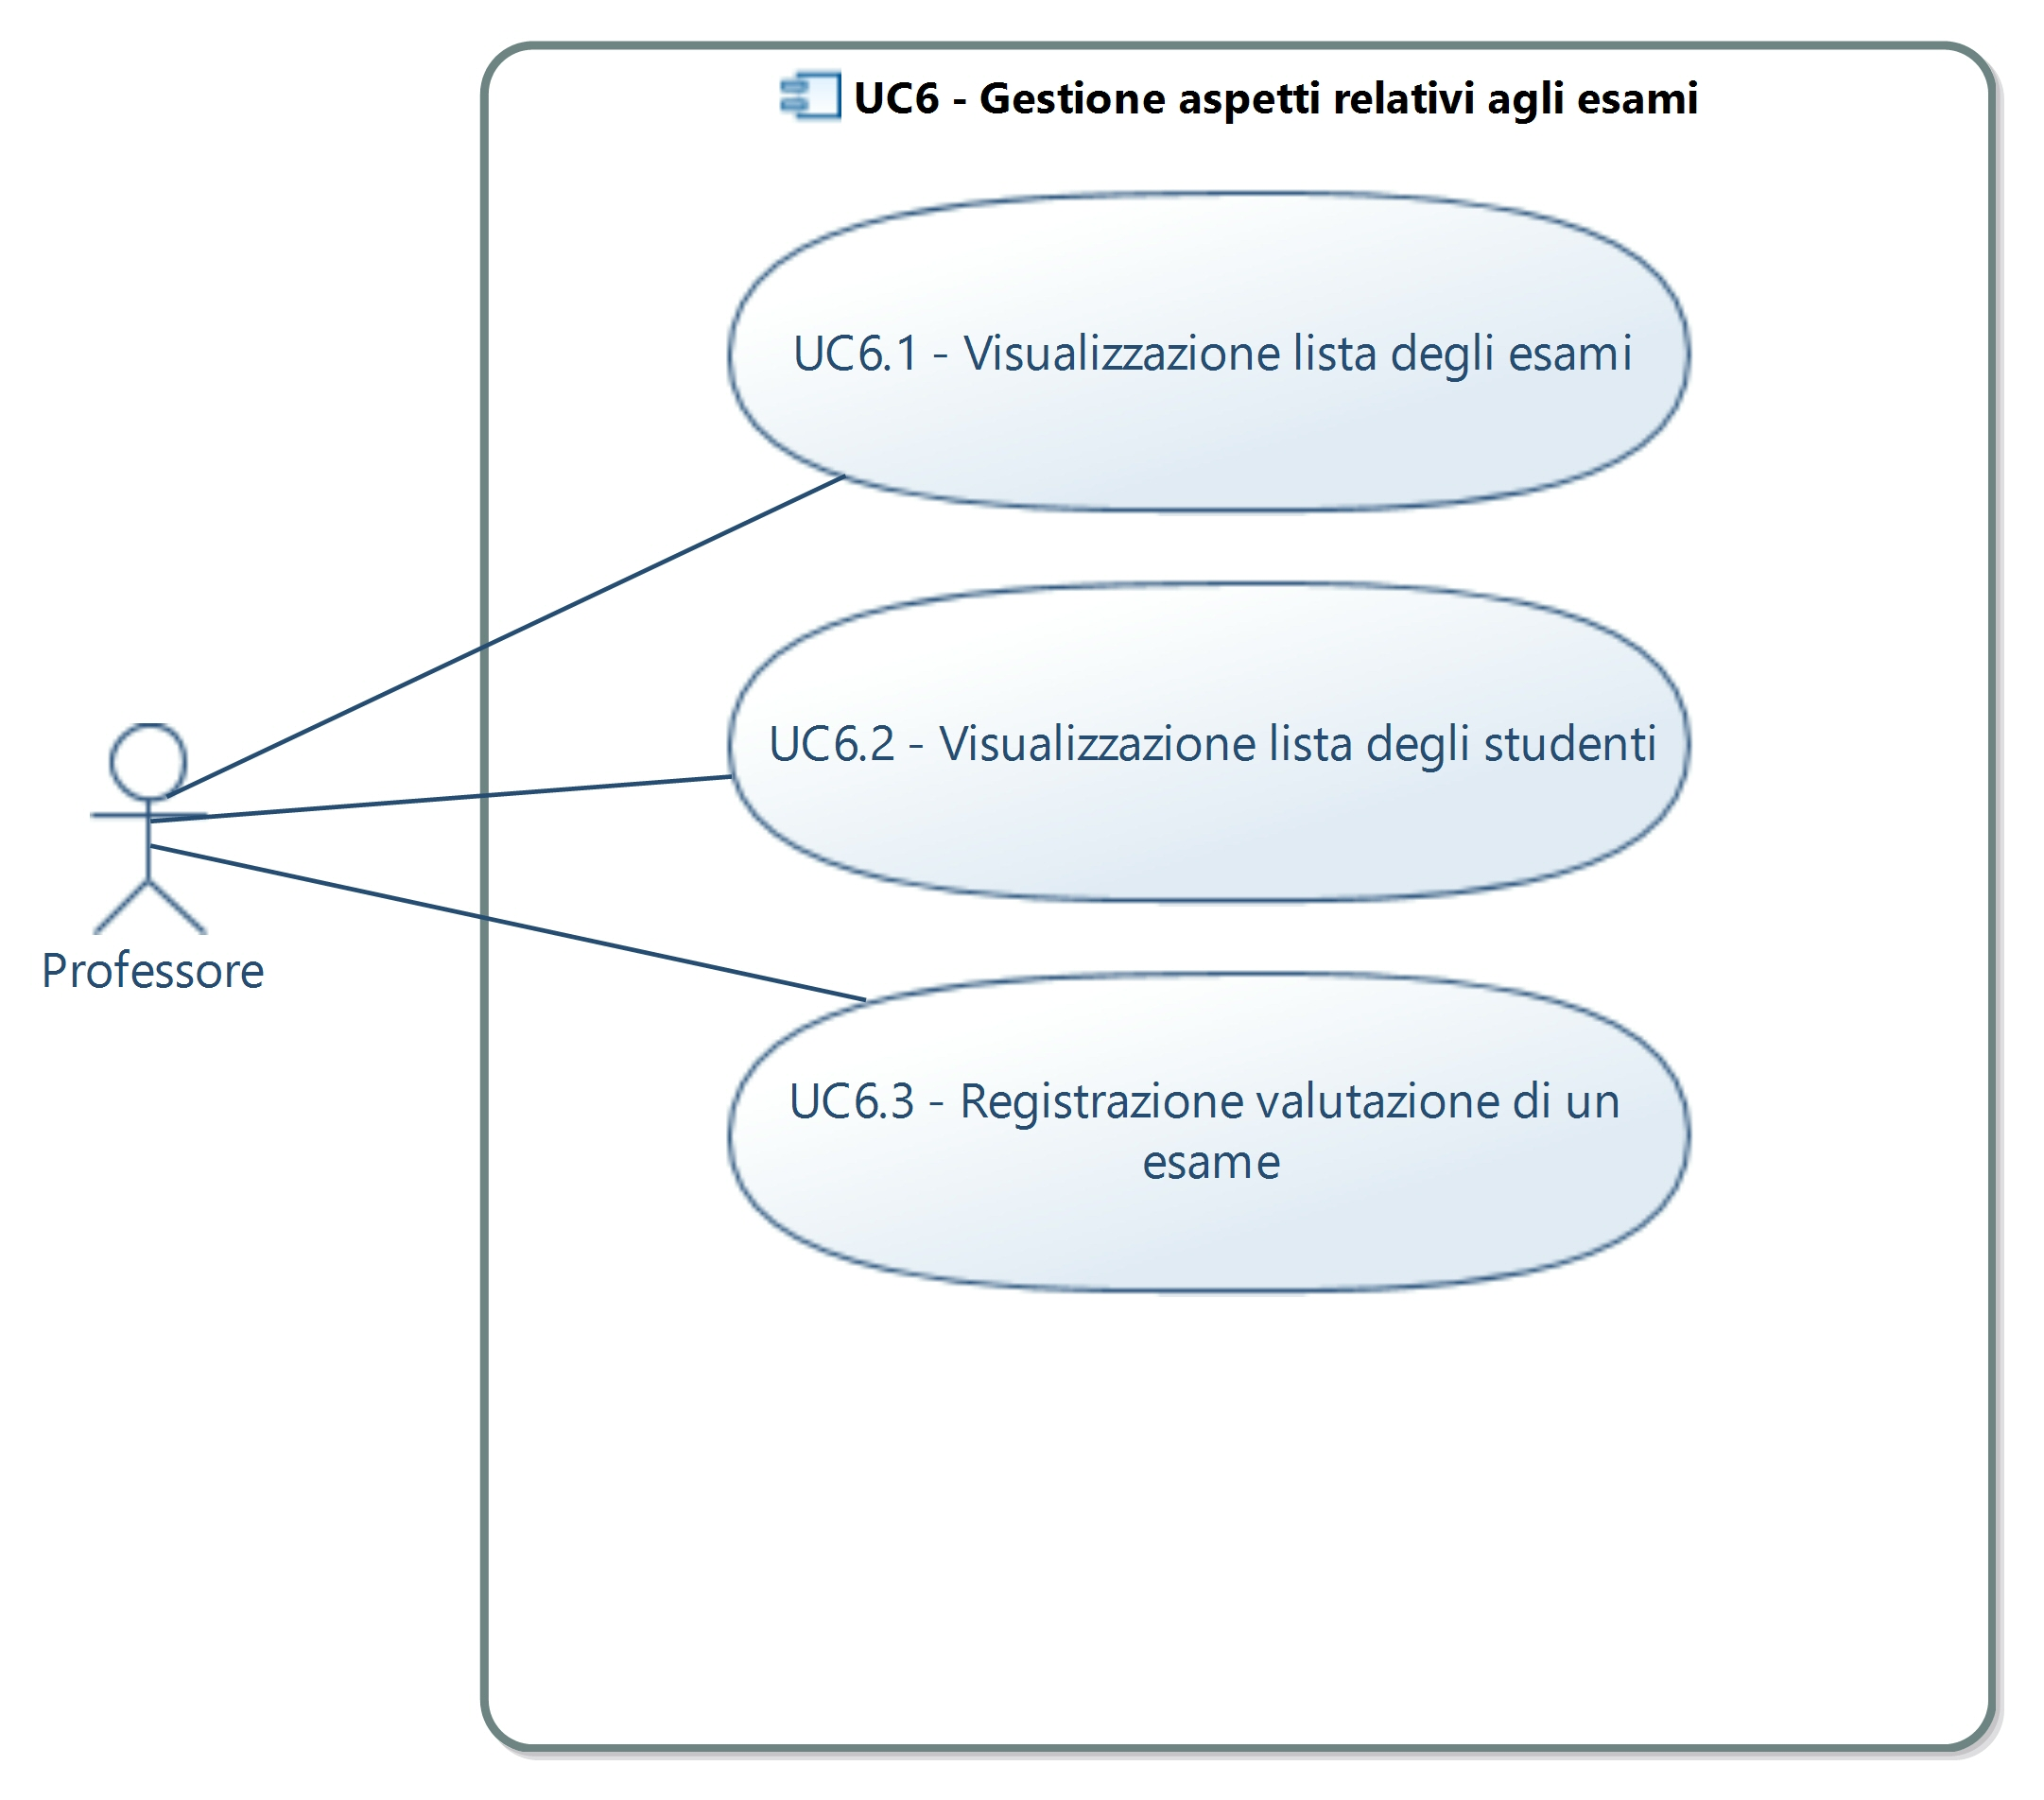
\includegraphics[width=0.8\linewidth]{UC6.jpg}
	\caption{UC6 - Gestione aspetti relativi agli esami}
	\label{fig:UC6 - Gestione aspetti relativi agli esami}
\end{figure}

\subsection{UC6.1 - Visualizzazione lista degli esami}
\begin{itemize}
	\item \textbf{Attori primari:} professore;\\
	\item \textbf{Scopo e descrizione:} il professore visualizza una lista di tutti gli esami ai quali è assegnato;\\
	\item \textbf{Scenario principale:} il professore richiede al sistema la lista degli esami di sua competenza per poterla consultare;\\
	\item \textbf{Precondizione:} l'utente è già riconosciuto dal sistema come professore e richiede la visualizzazione della lista degli esami di sua competenza;\\
	\item \textbf{Postcondizione:} il professore ottiene la lista degli esami ai quali è assegnato per poterla consultare.\\
\end{itemize}

\subsection{UC6.2 - Visualizzazione lista degli studenti}
\begin{itemize}
	\item \textbf{Attori primari:} professore;\\
	\item \textbf{Scopo e descrizione:} il professore visualizza una lista di tutti gli studenti iscritti ad un esame a lui assegnato;\\
	\item \textbf{Scenario principale:} il professore richiede al sistema la lista degli studenti iscritti ad un esami di sua competenza per poterla consultare;\\
	\item \textbf{Flusso principale degli eventi:}\\
	\begin{enumerate}
		\item il professore visualizza la lista degli esami di sua competenza [UC6.1];
		\item il professore, una volta individuato l'esame al quale è interessato, ne richiede la lista degli studenti registrati [UC6.2].
	\end{enumerate}
	\item \textbf{Precondizione:} l'utente è già riconosciuto dal sistema come professore e richiede la visualizzazione della lista degli studenti iscritti a un determinato esame di sua competenza;\\
	\item \textbf{Postcondizione:} il professore ottiene la lista degli studenti iscritti all'esame richiesto per poterla consultare.\\
\end{itemize}

\subsection{UC6.3 - Registrazione valutazione di un esame}
\begin{itemize}
	\item \textbf{Attori primari:} professore;\\
	\item \textbf{Scopo e descrizione:} il professore inserisce nel sistema una valutazione;\\
	\item \textbf{Flusso principale degli eventi:}\\
	\begin{enumerate}
		\item il professore visualizza la lista degli esami di sua competenza [UC6.1];
		\item il professore, una volta individuato l'esame al quale è interessato, ne richiede la lista degli studenti registrati [UC6.2];
		\item il professore consulta la lista degli studenti ed individua la persona alla quale deve inserire la valutazione [UC6.2];
		\item il professore inserisce la valutazione allo studente [UC6.3].
	\end{enumerate}
	\item \textbf{Precondizione:} il professore possiede una valutazione da assegnare a uno studente riguardante un determinato esame e desidera registrarlo;\\
	\item \textbf{Postcondizione:} il voto è stato inserito nella \citGloss{blockchain} universitaria.\\
%TODO discutere: nessuna estensione, vede solamente gli studenti dei suoi corsi, non può assegnare voti a studenti a caso di corsi a caso, se cerca di forzarlo modificando il js verrà bloccato dal contratto
\end{itemize}


\subsection{UC7 - Gestione aspetti relativi allo studente}
\begin{itemize}
	\item \textbf{Attori primari:} studente;\\
	\item \textbf{Attori secondari:} \citGloss{MetaMask};
	\item \textbf{Scopo e descrizione:} l'utente è già riconosciuto dal sistema come studente e sceglie di utilizzare una funzionalità messa a sua disposizione da parte del sistema;\\
	\item \textbf{Precondizione:} lo studente desidera effettuare delle operazioni relative alla scelta di esami opzionali o alla visione delle valutazioni;\\
	\item \textbf{Postcondizione:} lo studente ha visualizzato le operazioni messe a disposizione dal sistema e sceglie quale effettuare.\\
\end{itemize}

\begin{figure}[H]
	\centering
	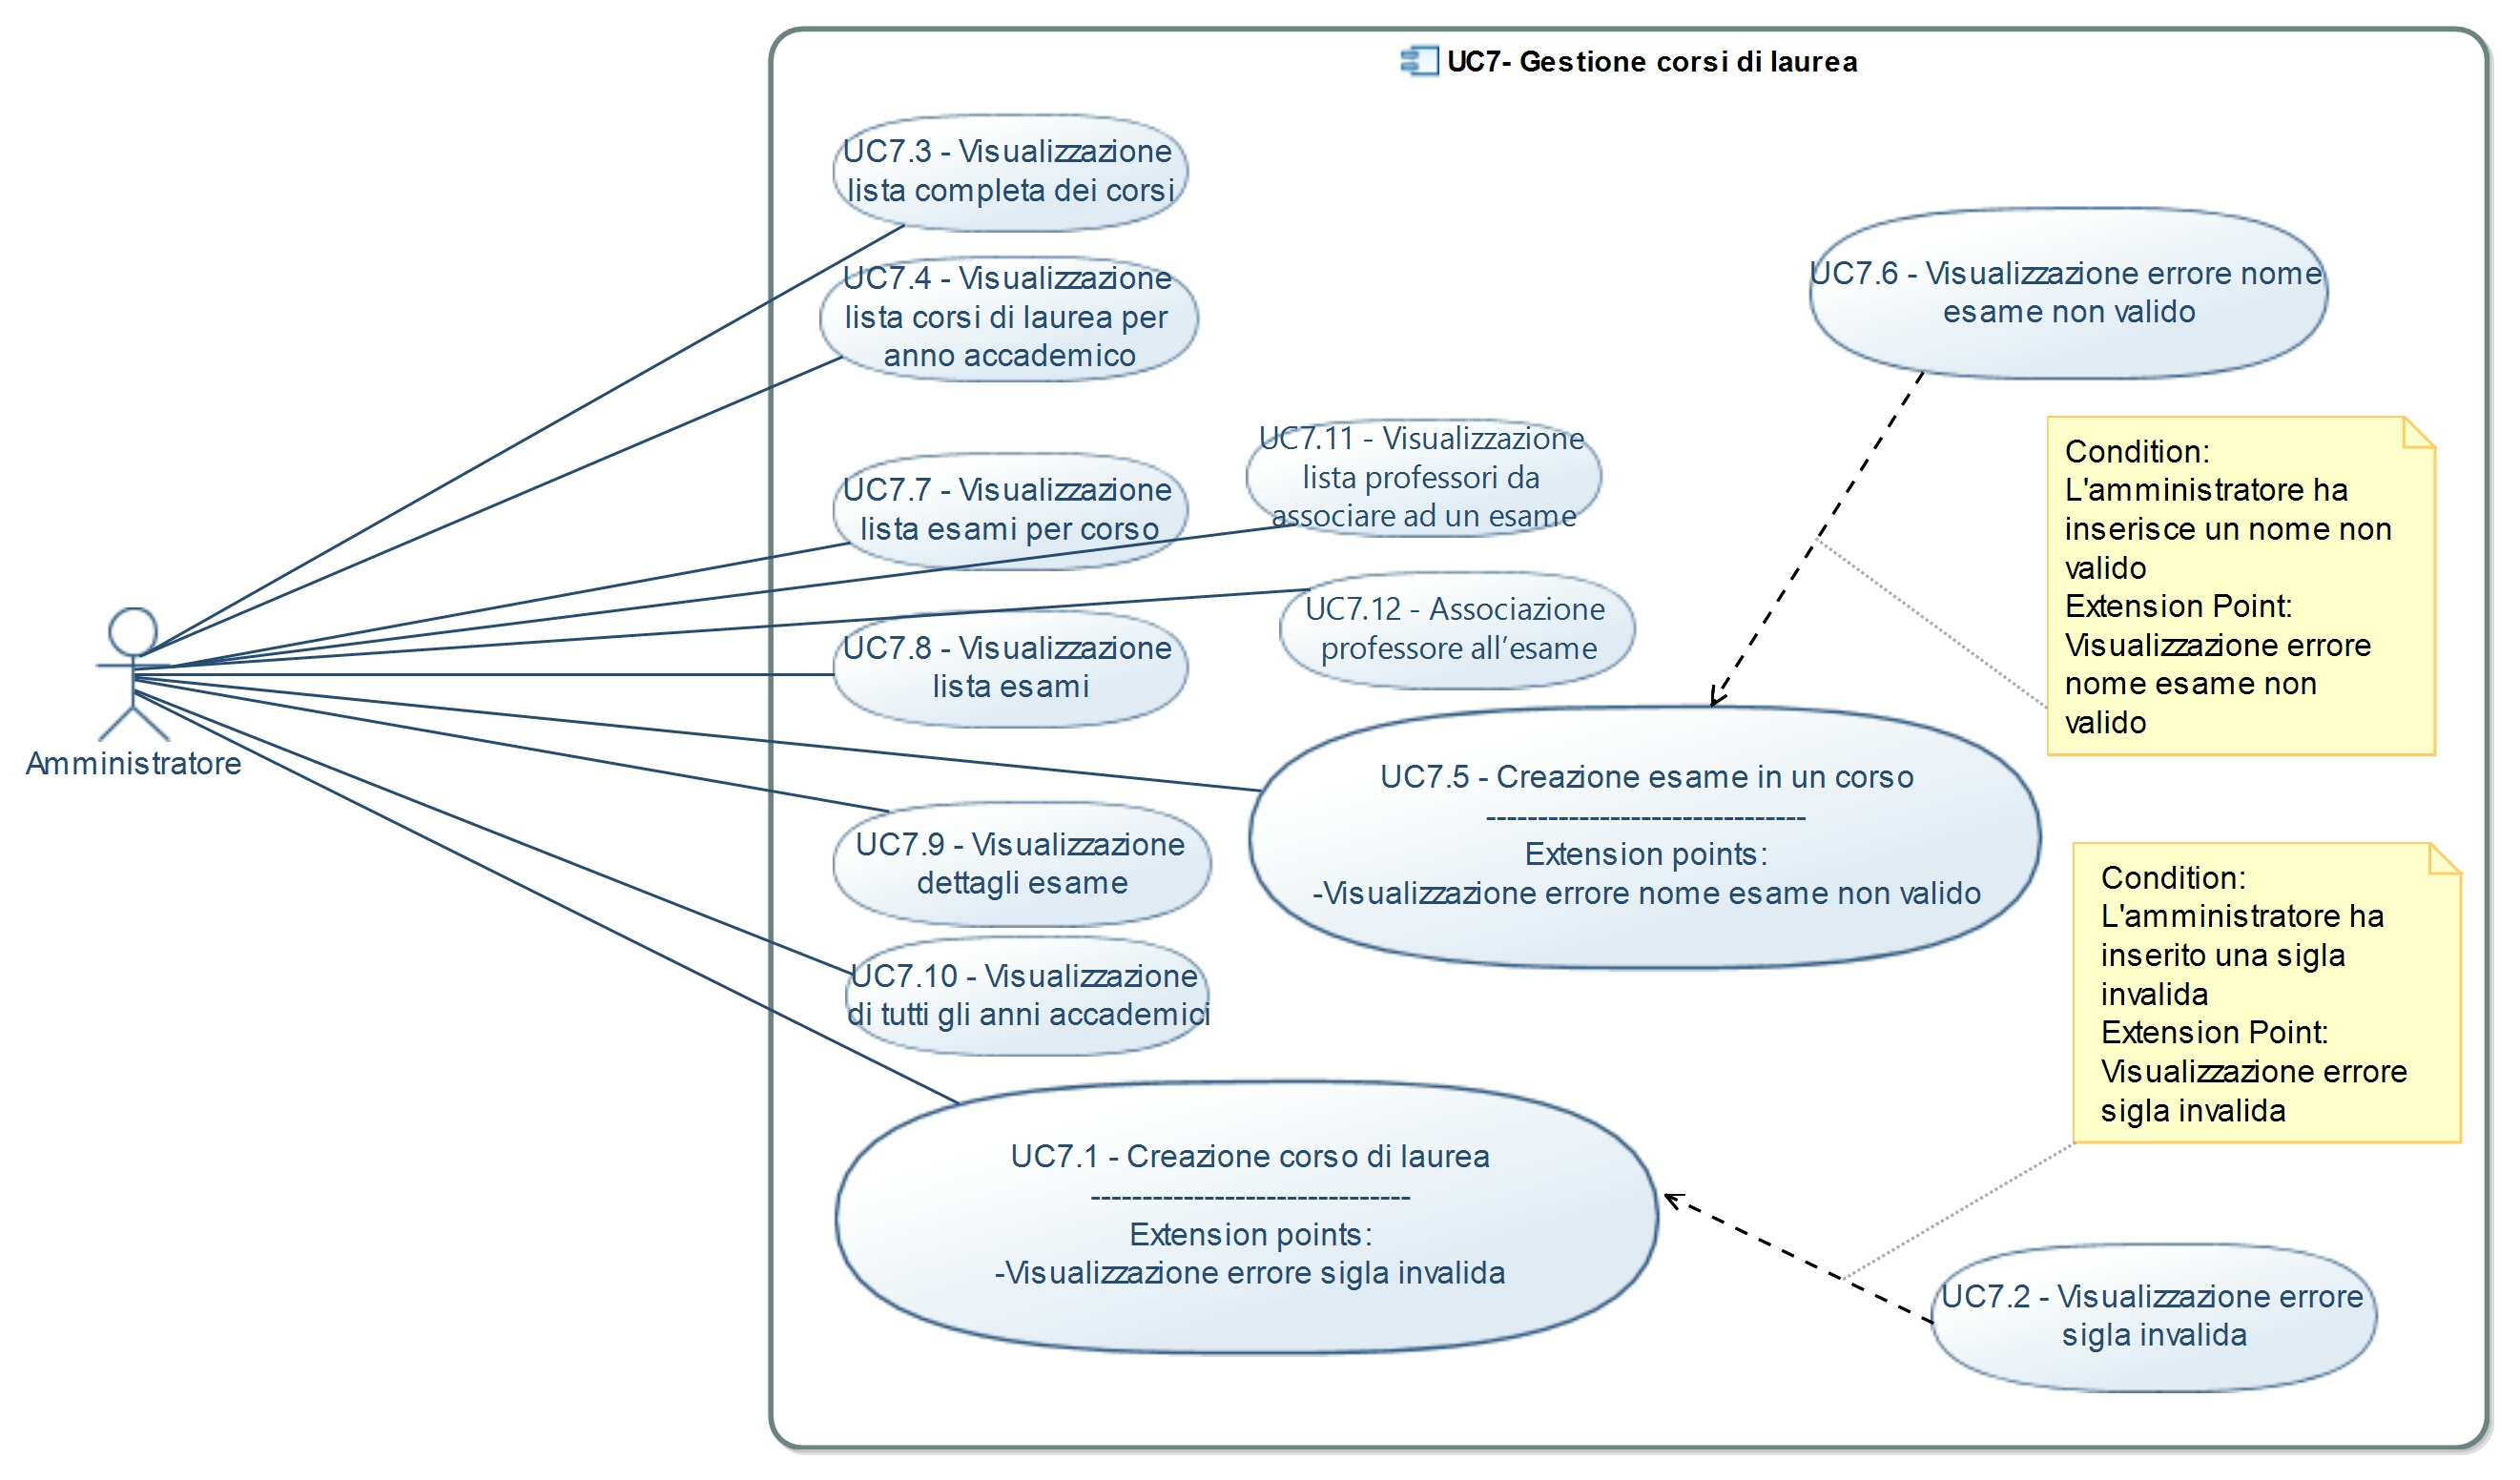
\includegraphics[width=0.8\linewidth]{UC7.jpg}
	\caption{UC7 - Gestione aspetti relativi allo studente}
	\label{fig:UC7 - Gestione aspetti relativi allo studente}
\end{figure}


\subsection{UC7.1 - Visualizzazione delle informazione degli esami ai quali è iscritto}
\begin{itemize}
	\item \textbf{Attori primari:} studente;\\
	\item \textbf{Scopo e descrizione:} lo studente visualizza una lista di tutti gli esami ai quali è iscritto;\\
	\item \textbf{Scenario principale:} lo studente richiede al sistema la lista degli esami ai quali è iscritto per poterla consultare;\\
	\item \textbf{Precondizione:} l'utente è già riconosciuto dal sistema come studente e richiede la visualizzazione della lista degli esami ai quali è iscritto ed le relative informazioni;\\
	\item \textbf{Postcondizione:} lo studente ottiene la lista per poterla consultare.\\
\end{itemize}

\begin{figure}[H]
	\centering
	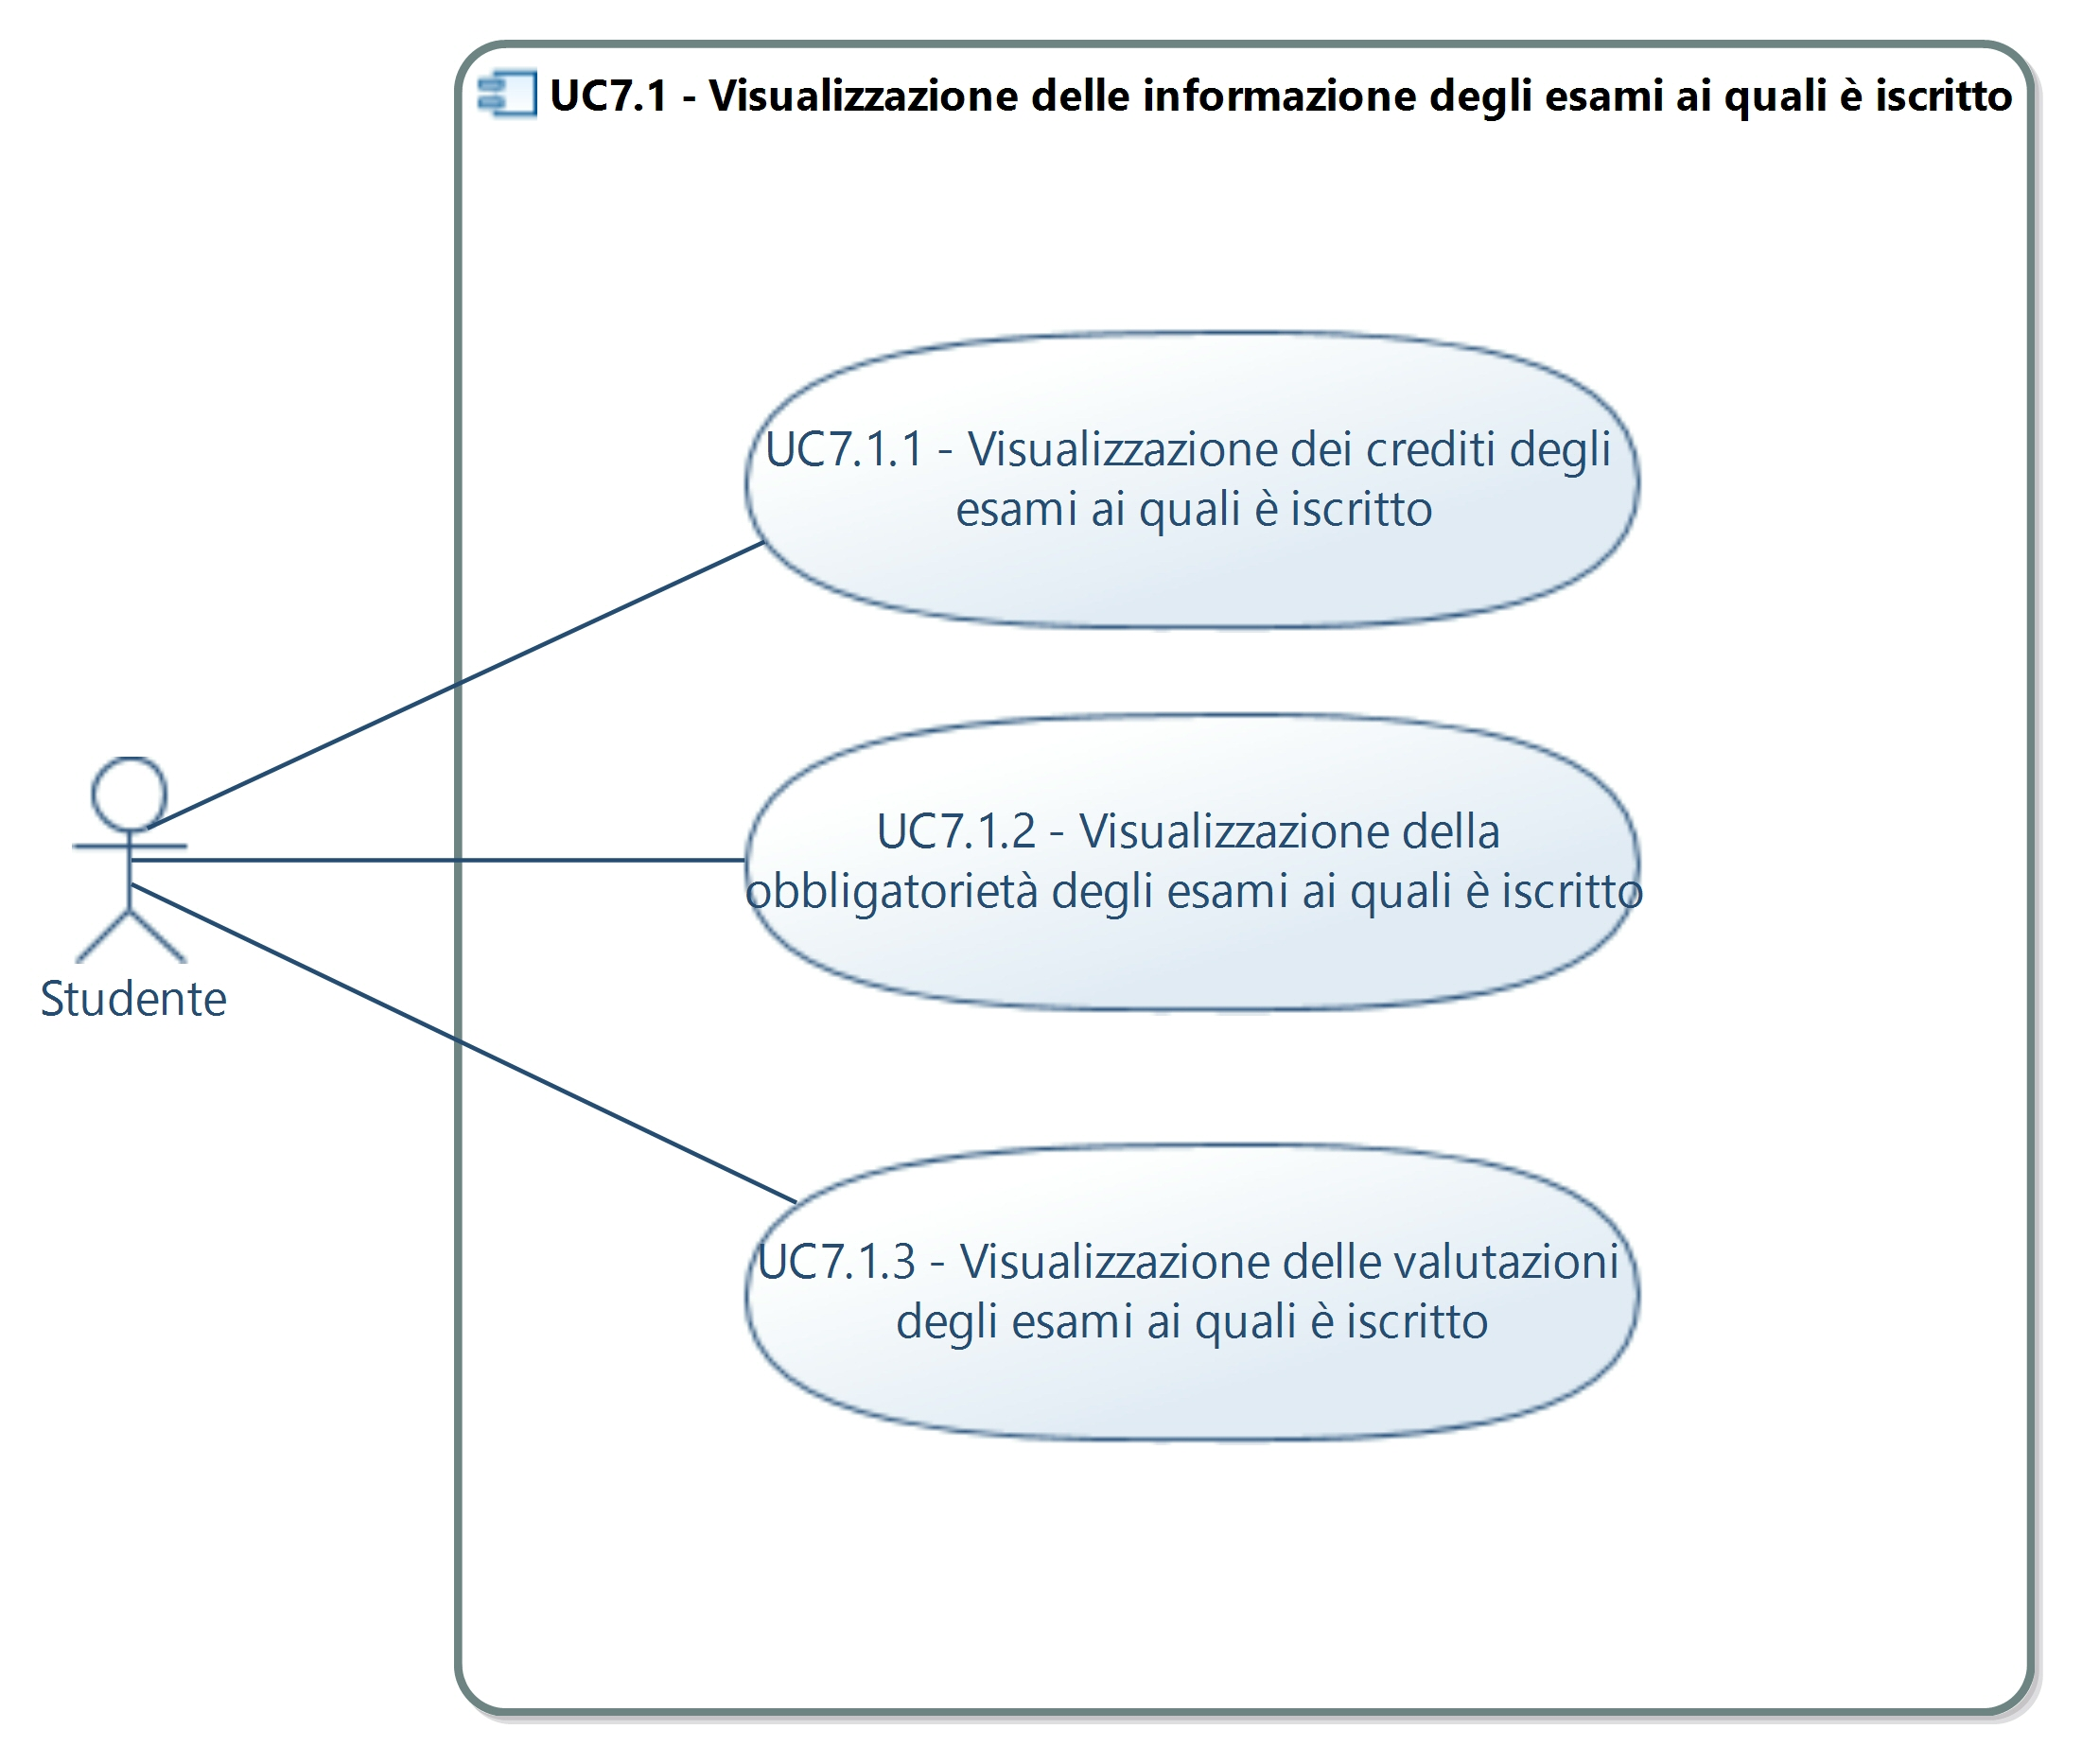
\includegraphics[width=1.0\linewidth]{UC7_1.jpg}
	\caption{UC7.1 - Visualizzazione delle informazione degli esami ai quali è iscritto}
	\label{fig:UC7.1 - Visualizzazione delle informazione degli esami ai quali e' iscritto} %TODO: aggiustare accenti nelle label
\end{figure}

\subsection{UC7.1.1 - Visualizzazione dei crediti degli esami ai quali è iscritto}
\begin{itemize}
\item \textbf{Attori primari:} studente;\\
\item \textbf{Scopo e descrizione:} lo studente visualizza il numero di crediti per ogni esame al quale è iscritto;\\
\item \textbf{Scenario principale:} lo studente richiede al sistema il numero di crediti degli esami ai quali è iscritto per consultarli;\\
\item \textbf{Precondizione:} l'utente è già riconosciuto dal sistema come studente e richiede il numero di crediti per ogni esame ai quale è iscritto;\\
\item \textbf{Postcondizione:} lo studente ottiene le informazioni richieste.\\
\end{itemize}

\subsection{UC7.1.2 - Visualizzazione della obbligatorietà degli esami ai quali è iscritto}
\begin{itemize}
	\item \textbf{Attori primari:} studente;\\
	\item \textbf{Scopo e descrizione:} lo studente visualizza il numero di crediti di per ogni esame al quale è iscritto;\\
	\item \textbf{Scenario principale:} lo studente richiede al sistema il numero di crediti degli esami ai quali è iscritto per consultarli;\\
	\item \textbf{Precondizione:} l'utente è già riconosciuto dal sistema come studente e richiede il numero di crediti per ogni esame ai quale è iscritto;\\
	\item \textbf{Postcondizione:} lo studente ottiene le informazioni richieste.\\
\end{itemize}

\subsection{UC7.1.3 - Visualizzazione delle valutazioni degli esami ai quali è iscritto}
\begin{itemize}
	\item \textbf{Attori primari:} studente;\\
	\item \textbf{Scopo e descrizione:} lo studente visualizza la valutazione, in formato numerico con l'indicazione di averlo superato se il voto è superiore a 18, per ogni esame al quale è iscritto;\\
	\item \textbf{Scenario principale:} lo studente richiede al sistema le informazioni riguardanti le valutazioni degli esami ai quali è iscritto per consultarle;\\
	\item \textbf{Precondizione:} l'utente è già riconosciuto dal sistema come studente e richiede le informazioni riguardanti le valutazioni degli esami ai quali è iscritto;\\
	\item \textbf{Postcondizione:} lo studente ottiene le informazioni richieste.\\
\end{itemize}

\subsection{UC7.2 - Visualizzazione degli esami opzionali e dei loro crediti}
\begin{itemize}
	\item \textbf{Attori primari:} studente;\\
	\item \textbf{Scopo e descrizione:} lo studente visualizza una lista di tutti gli esami opzionali ai quali ha possibilità di iscriversi ed i relativi crediti;\\
	\item \textbf{Scenario principale:} lo studente richiede al sistema la lista di tutti gli esami opzionali ai quali ha possibilità di iscriversi per poterla consultare con i relativi crediti;\\
	\item \textbf{Precondizione:} l'utente è già riconosciuto dal sistema come studente e richiede la visualizzazione della lista di tutti gli esami opzionali ai quali ha possibilità di iscriversi;\\
	\item \textbf{Postcondizione:} lo studente ottiene la lista per poterla consultare.\\
\end{itemize}

\subsection{UC7.3 - Registrazione ad un esame opzionale}
\begin{itemize}
	\item \textbf{Attori primari:} studente;\\
	\item \textbf{Scopo e descrizione:} lo studente si iscrive a un determinato esame opzionale;\\
	\item \textbf{Flusso principale degli eventi:}\\
	\begin{enumerate}
		\item lo studente visualizza la lista degli esami opzionali [UC7.2];
		\item lo studente individua l'esame al quale è interessato iscriversi;
		\item lo studente compie l'operazione di iscrizione;
	\end{enumerate}
	\item \textbf{Precondizione:} lo studente ha individuato l'esame opzionale al quale desidera iscriversi;\\
	\item \textbf{Postcondizione:} lo studente inserisce nella \citGloss{blockchain} universitaria l'iscrizione all'esame.\\
\end{itemize}

\subsection{UC7.4 - Visualizzazione delle informazioni relative ai crediti}
\begin{itemize}
	\item \textbf{Attori primari:} studente;\\
	\item \textbf{Scopo e descrizione:} lo studente visualizza un riepilogo del numero dei crediti che possiede e dell'obiettivo per poter conseguire la laurea;\\
	\item \textbf{Scenario principale:} lo studente richiede al sistema le informazioni riguardanti i suoi crediti;\\
	\item \textbf{Precondizione:} l'utente è già riconosciuto dal sistema come studente e richiede la visualizzazione delle informazioni relative ai suoi crediti;\\
	\item \textbf{Postcondizione:} lo studente ottiene le informazioni richieste per poterle consultare.\\
\end{itemize}
\subsection{UC8 - Gestione degli amministratori}
\begin{itemize}
	\item \textbf{Attori primari:} università;\\
	\item \textbf{Attori secondari:} \citGloss{MetaMask};
	\item \textbf{Scopo e descrizione:} l'utente è già riconosciuto dal sistema come rappresentante dell'università e sceglie di utilizzare una funzionalità messa a sua disposizione da parte del sistema;\\
	\item \textbf{Precondizione:} l'utente che rappresenta l'università desidera effettuare delle operazioni relative alla aggiunta o alla rimozione di amministratori;\\
	\item \textbf{Postcondizione:} l'utente che rappresenta l'università ha visualizzato le operazioni messe a disposizione dal sistema e sceglie quale effettuare.\\
\end{itemize}

\begin{figure}[H]
	\centering
	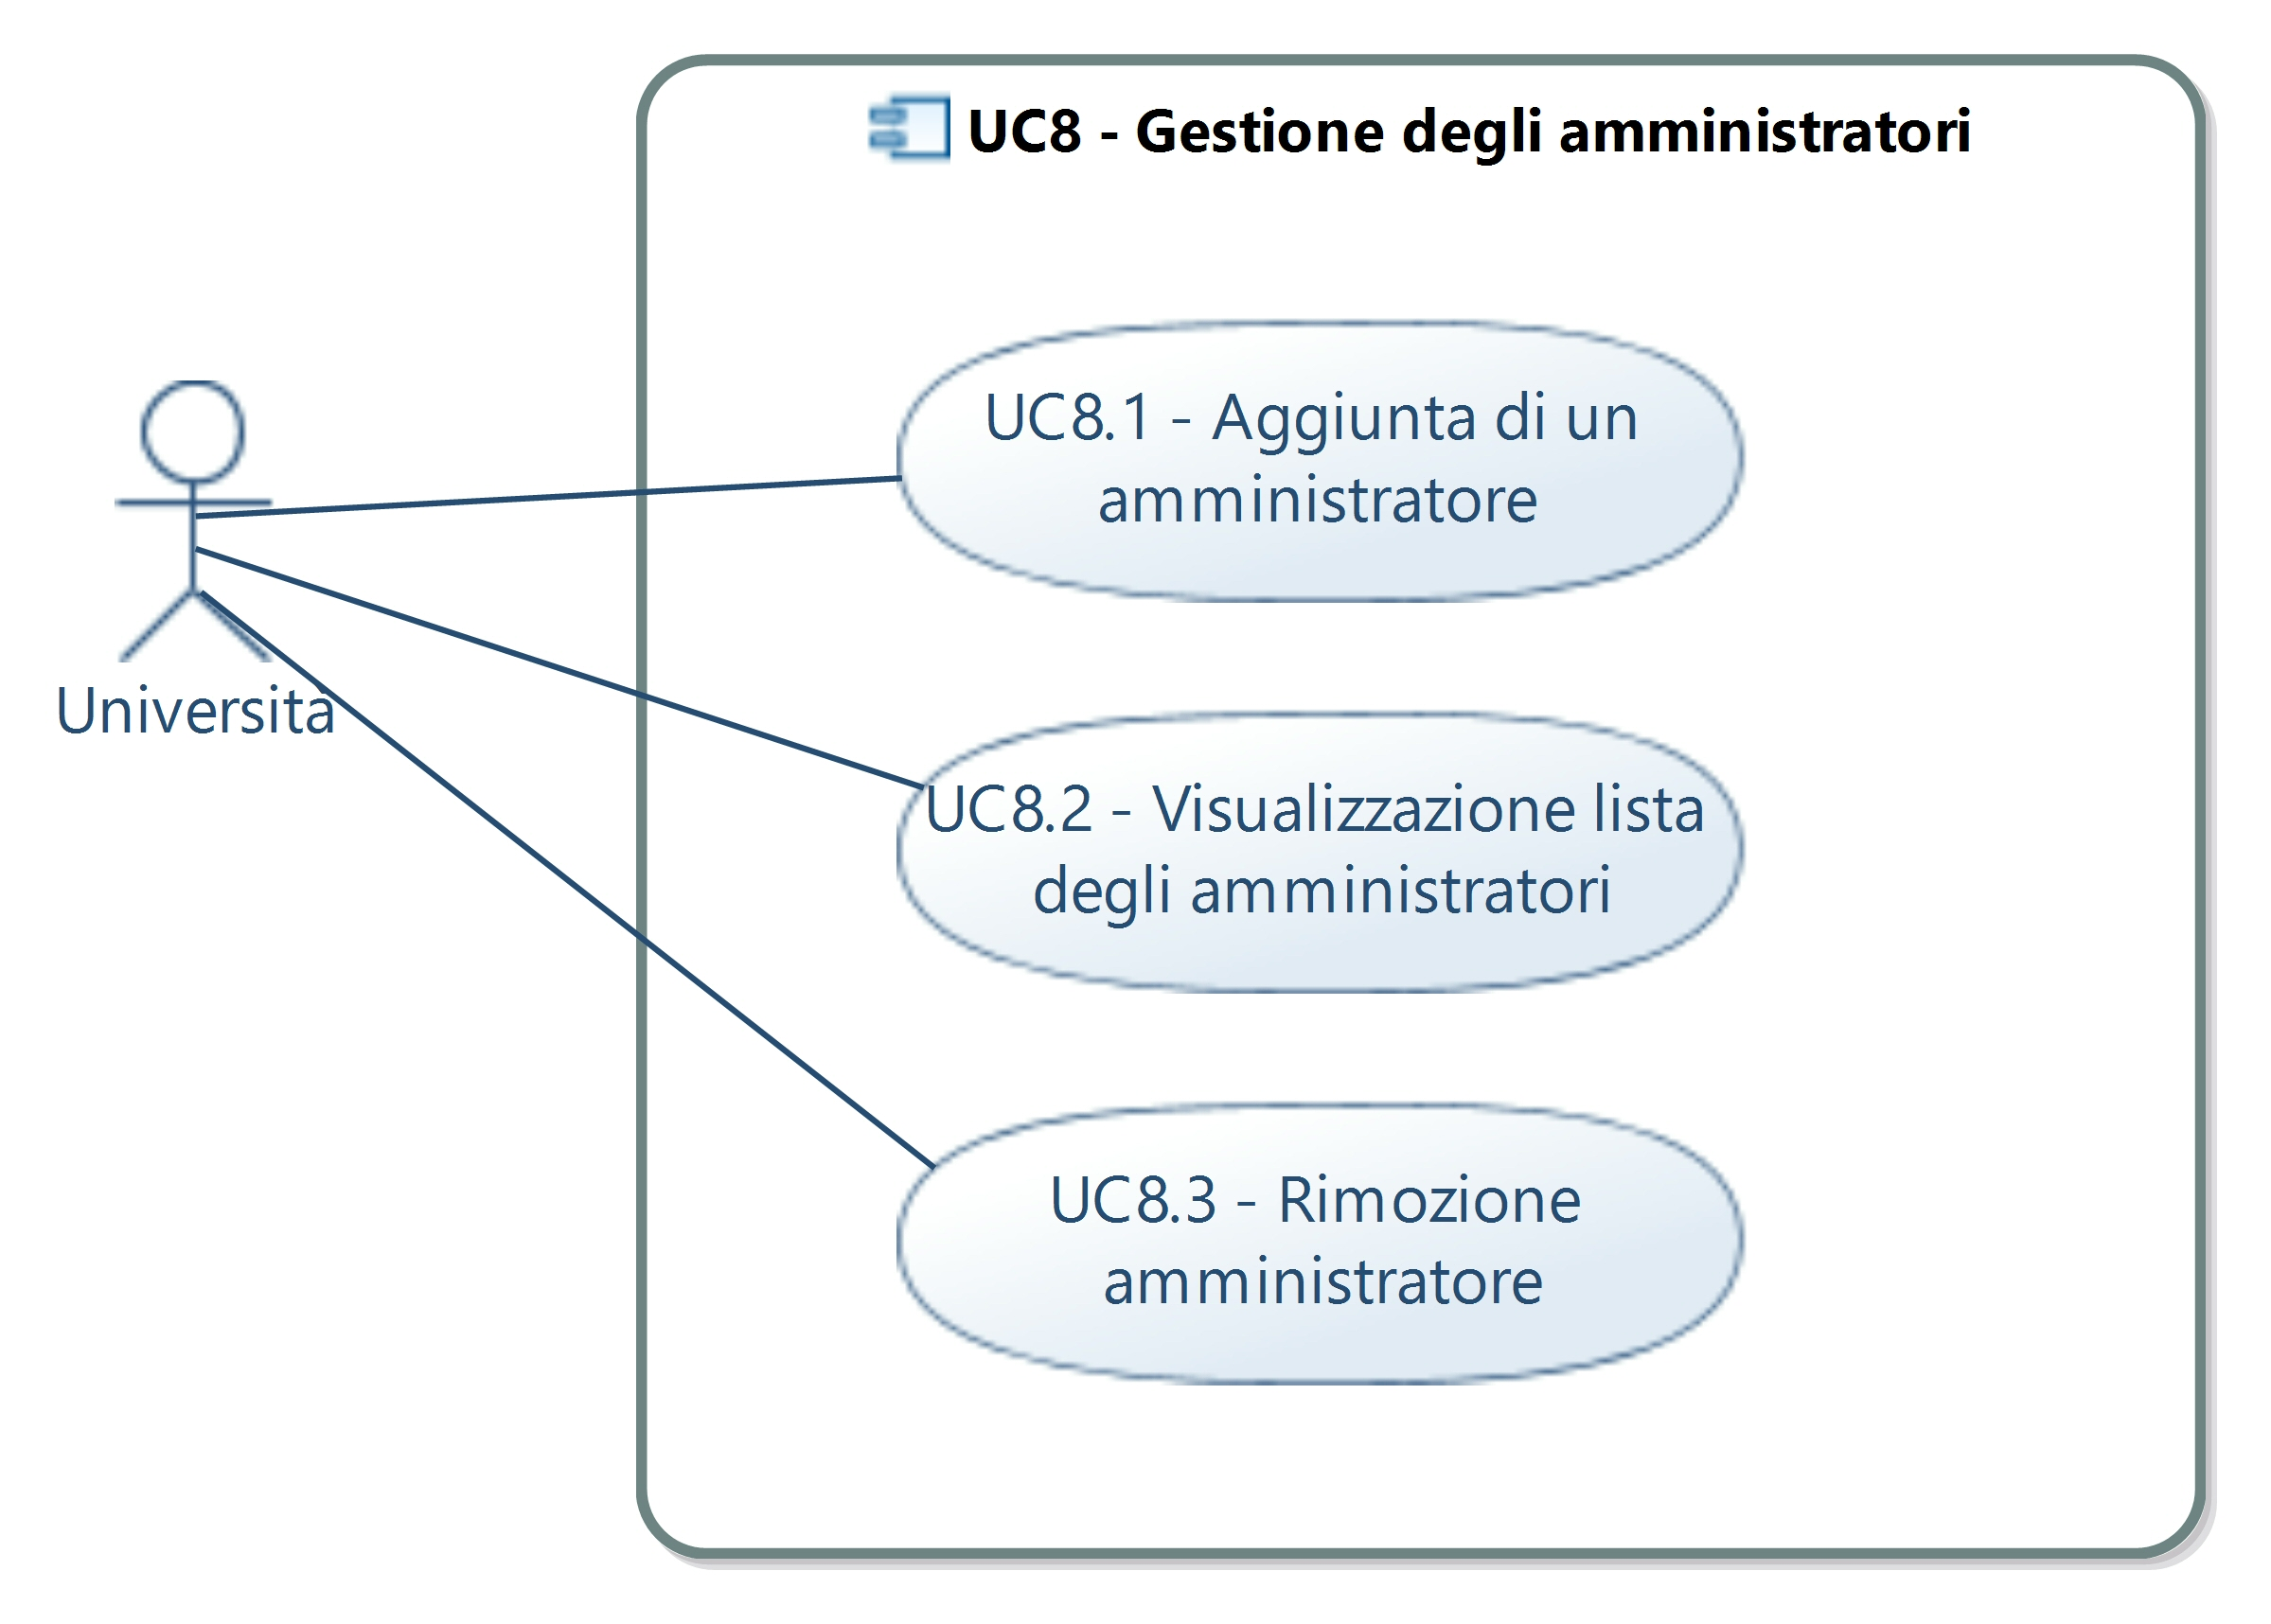
\includegraphics[width=1.0\linewidth]{UC8.jpg}
	\caption{UC8 - Gestione degli amministratori}
	\label{fig:UC8 - Gestione degli amministratori}
\end{figure}

\subsection{UC8.1 - Aggiunta di un amministratore}
\begin{itemize}
	\item \textbf{Attori primari:} università;\\
	\item \textbf{Scopo e descrizione:} l'utente che rappresenta l'università aggiunge un nuovo amministratore nel sistema;
	\item \textbf{Precondizione:} l'utente che rappresenta l'università ha scelto di aggiungere un nuovo amministratore; 
	\item \textbf{Postcondizione:} il nuovo amministratore è stato inserito nel sistema.
\end{itemize}

\begin{figure}[H]
	\centering
	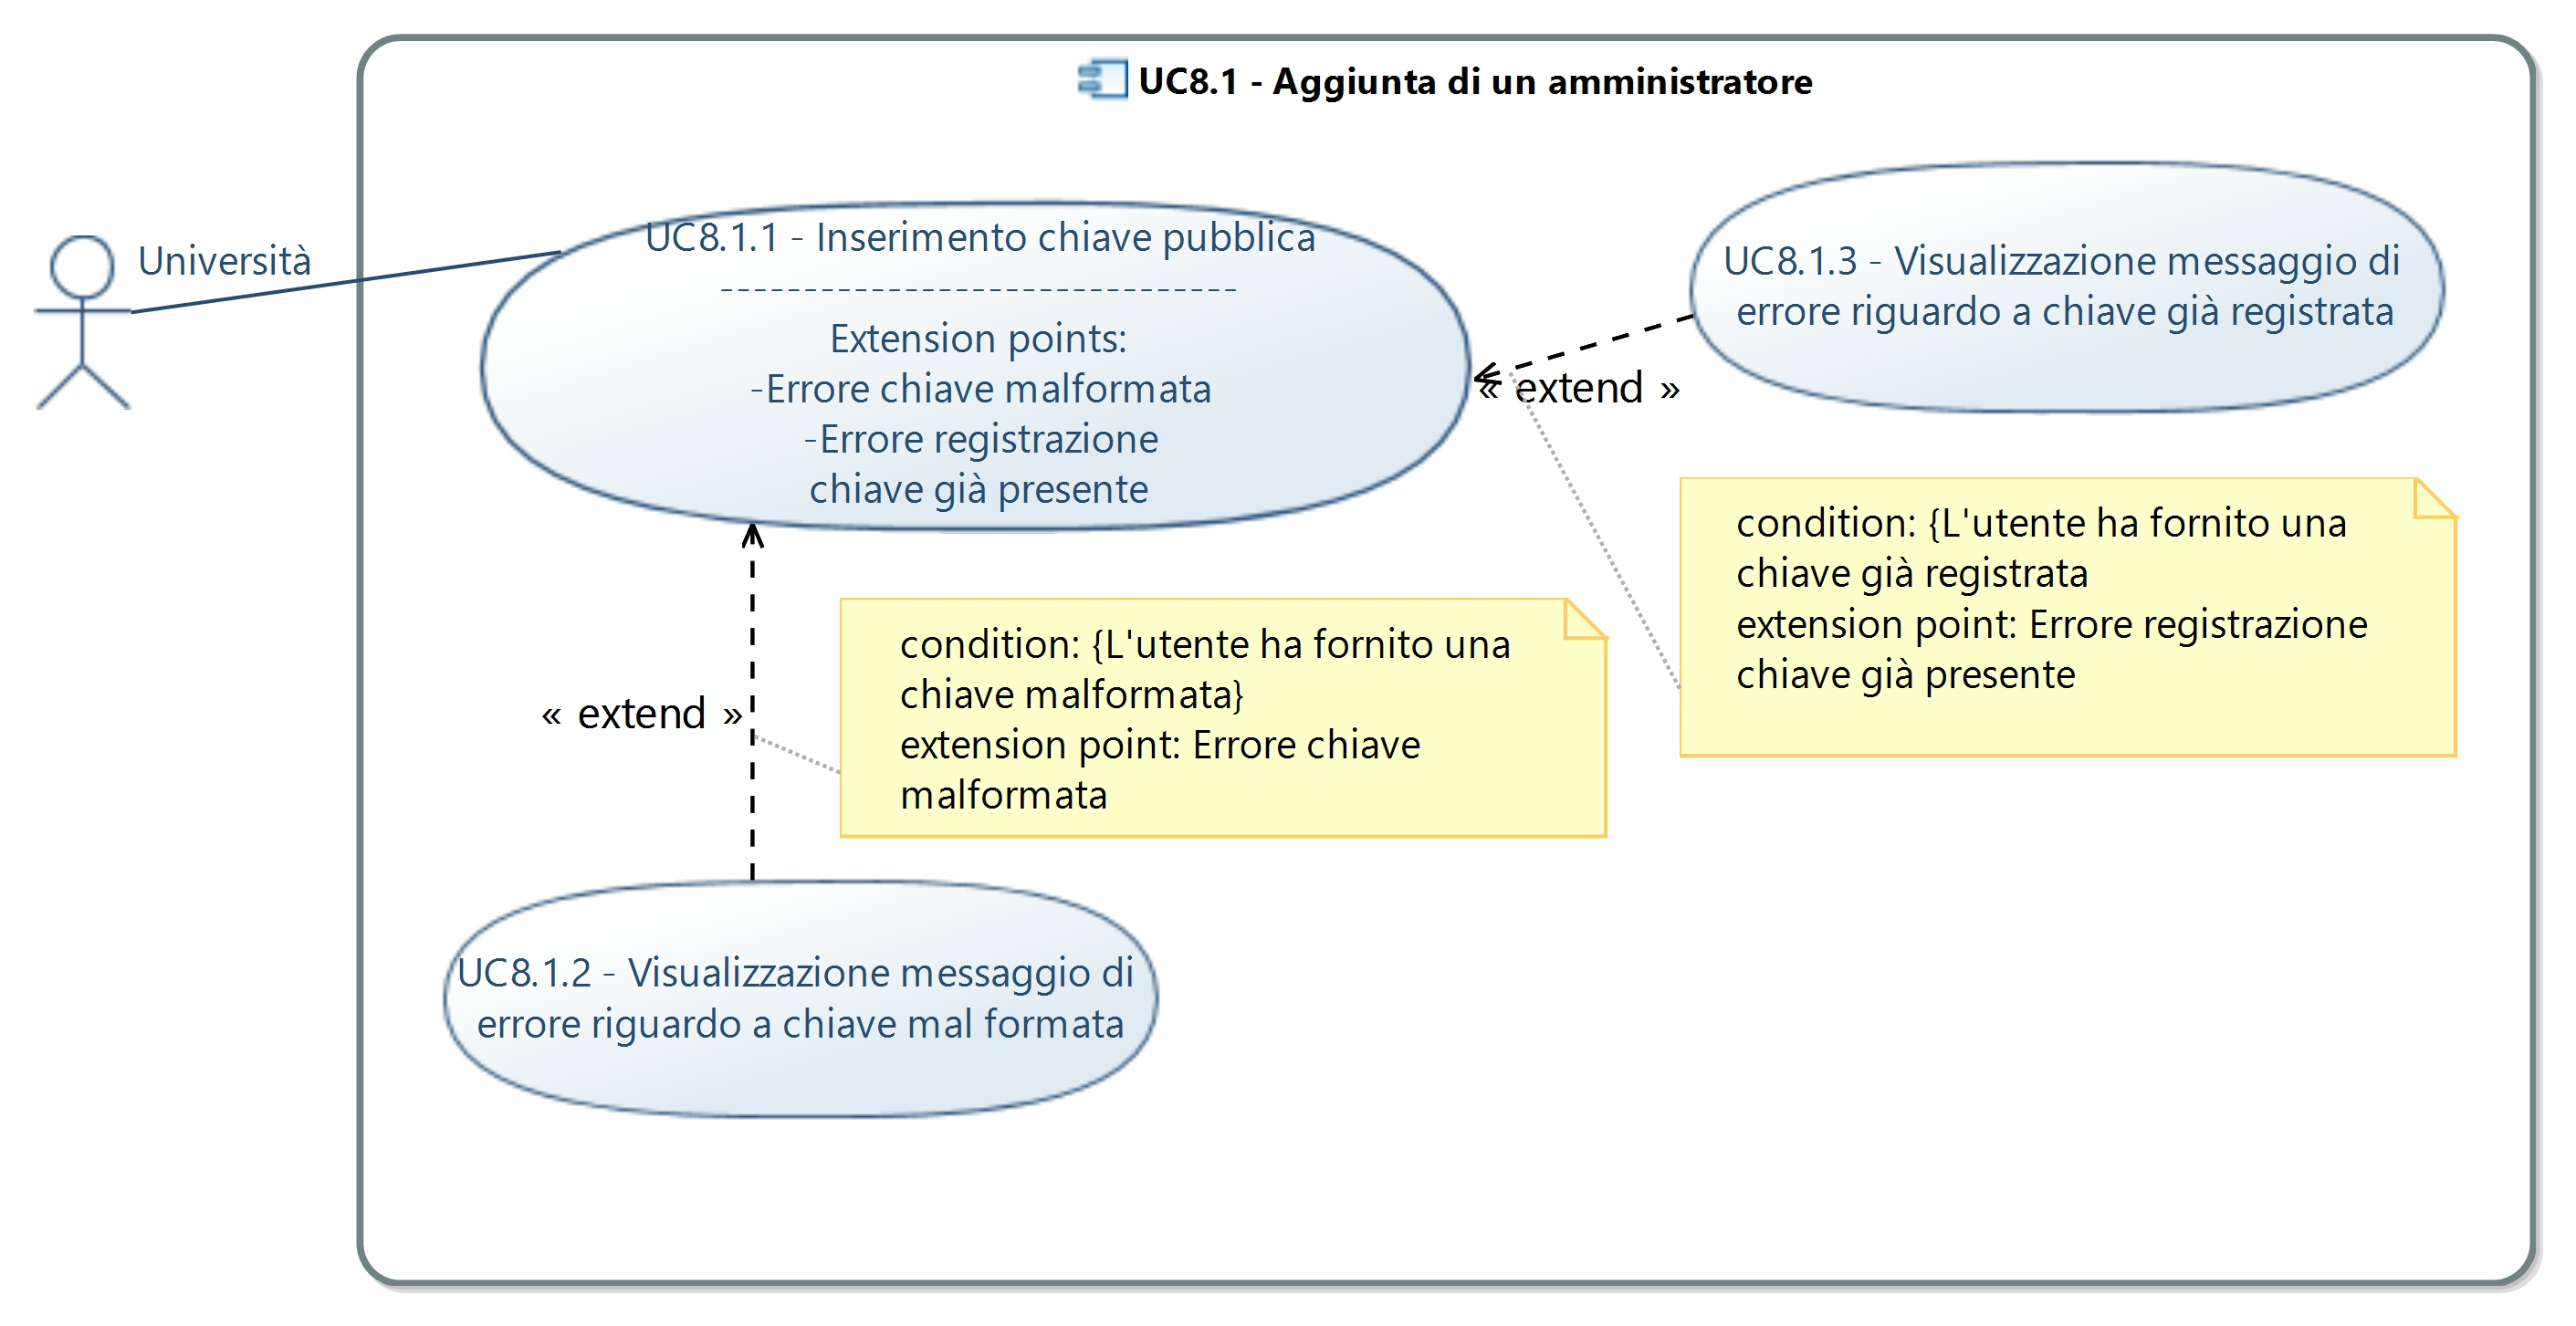
\includegraphics[width=1.0\linewidth]{UC8_1.jpg}
	\caption{UC8.1 - Aggiunta di un amministratore}
	\label{fig:UC8.1 - Aggiunta di un amministratore}
\end{figure}

\subsection{UC8.1.1 - Inserimento chiave pubblica}
\begin{itemize}
	\item \textbf{Attori primari:} università;\\
	\item \textbf{Scopo e Descrizione} il sistema offre l'interfaccia per inserire la \citGloss{chiave pubblica} del nuovo amministratore;
	\item \textbf{Scenario principale:} l'utente che rappresenta l'università fornisce tramite un dispositivo di input il suo nome;	\begin{enumerate}
		\item se la \citGloss{chiave pubblica} è mal formata l'utente viene avvisato con un relativo messaggio d'errore [UC8.1.2];
		\item se la \citGloss{chiave pubblica} è già registrata nel sistema in un altro ruolo l'utente viene avvisato un relativo messaggio d'errore [UC8.1.3].
	\end{enumerate}
	\item \textbf{Precondizione:} il sistema offre un campo per la compilazione della \citGloss{chiave pubblica} del nuovo amministratore e rimane in attesa dell'input;
	\item \textbf{Postcondizione:} l'utente che rappresenta l'università ha inserito la \citGloss{chiave pubblica} del nuovo amministratore nel campo fornito dal sistema;
\end{itemize}
\subsection{UC8.1.2 - Visualizzazione messaggio di errore riguardo a chiave mal formata}
\begin{itemize}
	\item \textbf{Attori primari:} università;\\
	\item \textbf{Scopo e descrizione:} l'utente viene avvisato del fatto che ha fornito una chiave ma formata, ad esempio di lunghezza invalida oppure non in caratteri esadecimali;\\
	\item \textbf{Scenario principale:} l'utente viene informato che la sua chiave risulta mal formata, invitandolo a ricontrollarla;\\
	\item \textbf{Precondizione:} l'utente cerca di registrare nel sistema una chiave mal formata;\\
	\item \textbf{Postcondizione:} l'utente è consapevole di aver tentato l'inserimento di una chiave mal formata.\\
\end{itemize}
\subsection{UC8.1.3 - Visualizzazione messaggio di errore riguardo a chiave già registrata}
\begin{itemize}
	\item \textbf{Attori primari:} università;\\
	\item \textbf{Scopo e descrizione:} l'utente viene avvisato del fatto che ha fornito una chiave già registrata in un altro ruolo all'interno dell'università;\\
	\item \textbf{Scenario principale:} l'utente viene informato che la sua chiave risulta già registrata;\\
	\item \textbf{Precondizione:} l'utente cerca di registrare nel sistema una chiave precedentemente registrata in un altro ruolo;\\
	\item \textbf{Postcondizione:} l'utente è consapevole di aver tentato l'inserimento di una chiave già registrata nell'università in un altro ruolo.\\
\end{itemize}


\subsection{UC8.2 - Visualizzazione lista degli amministratori}
	\begin{itemize}
	\item \textbf{Attori primari:} università;\\
	\item \textbf{Scopo e descrizione:} l'utente che rappresenta l'università visualizza una lista di tutti gli amministratori;\\
	\item \textbf{Scenario principale:} l'utente che rappresenta l'università richiede al sistema la lista degli amministratori per poterla consultare;\\
	\item \textbf{Precondizione:} l'utente che rappresenta l'università è già riconosciuto dal sistema come tale e richiede la visualizzazione della lista degli amministratori;\\
	\item \textbf{Postcondizione:} l'utente che rappresenta l'università ottiene la lista degli amministratori per poterla consultare.\\
	\end{itemize}
\subsection{UC8.3 - Rimozione amministratore}
\begin{itemize}
	\item \textbf{Attori primari:} università;\\
	\item \textbf{Scopo e descrizione:} l'utente che rappresenta l'università rimuove dal sistema un amministratore;\\
	\item \textbf{Flusso principale degli eventi:}\\
	\begin{enumerate}
		\item l'utente che rappresenta l'università  visualizza la lista degli amministratori [UC8.2];
		\item l'utente che rappresenta l'università, una volta ottenuta la lista degli amministratori, individua quale desidera rimuovere [UC8.2];\\
		\item l'utente che rappresenta l'università richiede al sistema l'eliminazione dell'amministratore [UC8.3].
	\end{enumerate}
	\item \textbf{Precondizione:} l'utente che rappresenta l'università desidera eliminare un amministratore dal sistema;\\
	\item \textbf{Postcondizione:} l'amministratore indicato viene rimosso dal ruolo nell'università e non può più autenticarsi come tale.\\
\end{itemize}

\subsection{UC9 - Visualizzazione quantità di Gas, Ether e costo delle operazioni}
\begin{itemize}
	\item \textbf{Attori primari:} ltente generico;\\
	\item \textbf{Attori secondari:} \citGloss{MetaMask};\\
	\item \textbf{Scopo e descrizione:} l'utente generico può vedere la quantità di \citGloss{Gas}, \citGloss{Ether} ed euro che andrà ad utilizzare per svolgere determinate azioni;\\
	\item \textbf{Precondizione:} l'utente generico desidera e richiede al sistema i costi delle operazioni;\\
	\item \textbf{Postcondizione:} il sistema fornisce all'utente generico le informazioni da lui richieste e l'utente generico acquisisce l'informazione.\\
\end{itemize}

\end{document}